\documentclass[]{article}
\usepackage{lmodern}
\usepackage{amssymb,amsmath}
\usepackage{ifxetex,ifluatex}
\usepackage{fixltx2e} % provides \textsubscript
\ifnum 0\ifxetex 1\fi\ifluatex 1\fi=0 % if pdftex
  \usepackage[T1]{fontenc}
  \usepackage[utf8]{inputenc}
\else % if luatex or xelatex
  \ifxetex
    \usepackage{mathspec}
  \else
    \usepackage{fontspec}
  \fi
  \defaultfontfeatures{Ligatures=TeX,Scale=MatchLowercase}
\fi
% use upquote if available, for straight quotes in verbatim environments
\IfFileExists{upquote.sty}{\usepackage{upquote}}{}
% use microtype if available
\IfFileExists{microtype.sty}{%
\usepackage{microtype}
\UseMicrotypeSet[protrusion]{basicmath} % disable protrusion for tt fonts
}{}
\usepackage[margin=1in]{geometry}
\usepackage{hyperref}
\hypersetup{unicode=true,
            pdftitle={Linear model fit for p-value discrepancies},
            pdfborder={0 0 0},
            breaklinks=true}
\urlstyle{same}  % don't use monospace font for urls
\usepackage{color}
\usepackage{fancyvrb}
\newcommand{\VerbBar}{|}
\newcommand{\VERB}{\Verb[commandchars=\\\{\}]}
\DefineVerbatimEnvironment{Highlighting}{Verbatim}{commandchars=\\\{\}}
% Add ',fontsize=\small' for more characters per line
\usepackage{framed}
\definecolor{shadecolor}{RGB}{248,248,248}
\newenvironment{Shaded}{\begin{snugshade}}{\end{snugshade}}
\newcommand{\KeywordTok}[1]{\textcolor[rgb]{0.13,0.29,0.53}{\textbf{#1}}}
\newcommand{\DataTypeTok}[1]{\textcolor[rgb]{0.13,0.29,0.53}{#1}}
\newcommand{\DecValTok}[1]{\textcolor[rgb]{0.00,0.00,0.81}{#1}}
\newcommand{\BaseNTok}[1]{\textcolor[rgb]{0.00,0.00,0.81}{#1}}
\newcommand{\FloatTok}[1]{\textcolor[rgb]{0.00,0.00,0.81}{#1}}
\newcommand{\ConstantTok}[1]{\textcolor[rgb]{0.00,0.00,0.00}{#1}}
\newcommand{\CharTok}[1]{\textcolor[rgb]{0.31,0.60,0.02}{#1}}
\newcommand{\SpecialCharTok}[1]{\textcolor[rgb]{0.00,0.00,0.00}{#1}}
\newcommand{\StringTok}[1]{\textcolor[rgb]{0.31,0.60,0.02}{#1}}
\newcommand{\VerbatimStringTok}[1]{\textcolor[rgb]{0.31,0.60,0.02}{#1}}
\newcommand{\SpecialStringTok}[1]{\textcolor[rgb]{0.31,0.60,0.02}{#1}}
\newcommand{\ImportTok}[1]{#1}
\newcommand{\CommentTok}[1]{\textcolor[rgb]{0.56,0.35,0.01}{\textit{#1}}}
\newcommand{\DocumentationTok}[1]{\textcolor[rgb]{0.56,0.35,0.01}{\textbf{\textit{#1}}}}
\newcommand{\AnnotationTok}[1]{\textcolor[rgb]{0.56,0.35,0.01}{\textbf{\textit{#1}}}}
\newcommand{\CommentVarTok}[1]{\textcolor[rgb]{0.56,0.35,0.01}{\textbf{\textit{#1}}}}
\newcommand{\OtherTok}[1]{\textcolor[rgb]{0.56,0.35,0.01}{#1}}
\newcommand{\FunctionTok}[1]{\textcolor[rgb]{0.00,0.00,0.00}{#1}}
\newcommand{\VariableTok}[1]{\textcolor[rgb]{0.00,0.00,0.00}{#1}}
\newcommand{\ControlFlowTok}[1]{\textcolor[rgb]{0.13,0.29,0.53}{\textbf{#1}}}
\newcommand{\OperatorTok}[1]{\textcolor[rgb]{0.81,0.36,0.00}{\textbf{#1}}}
\newcommand{\BuiltInTok}[1]{#1}
\newcommand{\ExtensionTok}[1]{#1}
\newcommand{\PreprocessorTok}[1]{\textcolor[rgb]{0.56,0.35,0.01}{\textit{#1}}}
\newcommand{\AttributeTok}[1]{\textcolor[rgb]{0.77,0.63,0.00}{#1}}
\newcommand{\RegionMarkerTok}[1]{#1}
\newcommand{\InformationTok}[1]{\textcolor[rgb]{0.56,0.35,0.01}{\textbf{\textit{#1}}}}
\newcommand{\WarningTok}[1]{\textcolor[rgb]{0.56,0.35,0.01}{\textbf{\textit{#1}}}}
\newcommand{\AlertTok}[1]{\textcolor[rgb]{0.94,0.16,0.16}{#1}}
\newcommand{\ErrorTok}[1]{\textcolor[rgb]{0.64,0.00,0.00}{\textbf{#1}}}
\newcommand{\NormalTok}[1]{#1}
\usepackage{graphicx,grffile}
\makeatletter
\def\maxwidth{\ifdim\Gin@nat@width>\linewidth\linewidth\else\Gin@nat@width\fi}
\def\maxheight{\ifdim\Gin@nat@height>\textheight\textheight\else\Gin@nat@height\fi}
\makeatother
% Scale images if necessary, so that they will not overflow the page
% margins by default, and it is still possible to overwrite the defaults
% using explicit options in \includegraphics[width, height, ...]{}
\setkeys{Gin}{width=\maxwidth,height=\maxheight,keepaspectratio}
\IfFileExists{parskip.sty}{%
\usepackage{parskip}
}{% else
\setlength{\parindent}{0pt}
\setlength{\parskip}{6pt plus 2pt minus 1pt}
}
\setlength{\emergencystretch}{3em}  % prevent overfull lines
\providecommand{\tightlist}{%
  \setlength{\itemsep}{0pt}\setlength{\parskip}{0pt}}
\setcounter{secnumdepth}{0}
% Redefines (sub)paragraphs to behave more like sections
\ifx\paragraph\undefined\else
\let\oldparagraph\paragraph
\renewcommand{\paragraph}[1]{\oldparagraph{#1}\mbox{}}
\fi
\ifx\subparagraph\undefined\else
\let\oldsubparagraph\subparagraph
\renewcommand{\subparagraph}[1]{\oldsubparagraph{#1}\mbox{}}
\fi

%%% Use protect on footnotes to avoid problems with footnotes in titles
\let\rmarkdownfootnote\footnote%
\def\footnote{\protect\rmarkdownfootnote}

%%% Change title format to be more compact
\usepackage{titling}

% Create subtitle command for use in maketitle
\providecommand{\subtitle}[1]{
  \posttitle{
    \begin{center}\large#1\end{center}
    }
}

\setlength{\droptitle}{-2em}

  \title{Linear model fit for p-value discrepancies}
    \pretitle{\vspace{\droptitle}\centering\huge}
  \posttitle{\par}
    \author{}
    \preauthor{}\postauthor{}
    \date{}
    \predate{}\postdate{}
  

\begin{document}
\maketitle

\begin{Shaded}
\begin{Highlighting}[]
\NormalTok{rasq =}\StringTok{ }\KeywordTok{read.csv}\NormalTok{(}\StringTok{"linear_model_cov.csv"}\NormalTok{)}
\NormalTok{rasq =}\StringTok{ }\NormalTok{rasq[}\OperatorTok{!}\KeywordTok{is.na}\NormalTok{(rasq}\OperatorTok{$}\NormalTok{pvalT),]}
\NormalTok{rasq}\OperatorTok{$}\NormalTok{qvalR =}\StringTok{ }\DecValTok{10}\OperatorTok{^}\NormalTok{rasq}\OperatorTok{$}\NormalTok{qval}
\NormalTok{rasq}\OperatorTok{$}\NormalTok{qvalT[rasq}\OperatorTok{$}\NormalTok{qvalT}\OperatorTok{<}\FloatTok{1e-100}\NormalTok{] =}\StringTok{ }\FloatTok{1e-100}
\NormalTok{rasq}\OperatorTok{$}\NormalTok{qvalR[rasq}\OperatorTok{$}\NormalTok{qvalR}\OperatorTok{<}\FloatTok{1e-100}\NormalTok{] =}\StringTok{ }\FloatTok{1e-100}

\CommentTok{#rasq$rnlt = -log10(rasq$qvalR)}
\CommentTok{#rasq$tnlt = -log10(rasq$qvalT)}
\NormalTok{rasq}\OperatorTok{$}\NormalTok{rnlt =}\StringTok{ }\OperatorTok{-}\KeywordTok{log10}\NormalTok{(rasq}\OperatorTok{$}\NormalTok{pvalR)}
\NormalTok{rasq}\OperatorTok{$}\NormalTok{tnlt =}\StringTok{ }\OperatorTok{-}\KeywordTok{log10}\NormalTok{(rasq}\OperatorTok{$}\NormalTok{pvalT)}

\NormalTok{cent =}\StringTok{ }\ControlFlowTok{function}\NormalTok{(x)\{}
\NormalTok{  med =}\StringTok{ }\KeywordTok{median}\NormalTok{(x)}
\NormalTok{  (x}\OperatorTok{-}\NormalTok{med)}
\NormalTok{\}}
\NormalTok{norm =}\StringTok{ }\ControlFlowTok{function}\NormalTok{(x)\{}
\NormalTok{  sd =}\StringTok{ }\KeywordTok{sd}\NormalTok{(x)}
\NormalTok{  x}\OperatorTok{/}\NormalTok{sd}
\NormalTok{\}}

\NormalTok{odNB =}\StringTok{ }\NormalTok{rasq}\OperatorTok{$}\NormalTok{odNB; odNB[odNB}\OperatorTok{<}\FloatTok{1e-3}\NormalTok{]=}\FloatTok{1e-3}\NormalTok{; odNB[odNB}\OperatorTok{>}\DecValTok{8}\NormalTok{]=}\DecValTok{8}\NormalTok{; }
\NormalTok{odBB =}\StringTok{ }\NormalTok{rasq}\OperatorTok{$}\NormalTok{odBB; odBB[odBB}\OperatorTok{<}\FloatTok{1e-3}\NormalTok{]=}\FloatTok{1e-3}\NormalTok{; odBB[odBB}\OperatorTok{>}\DecValTok{8}\NormalTok{]=}\DecValTok{8}
\NormalTok{lodNB =}\StringTok{ }\KeywordTok{cent}\NormalTok{(}\KeywordTok{norm}\NormalTok{(}\KeywordTok{log}\NormalTok{(odNB))); }
\NormalTok{lodBB =}\StringTok{ }\KeywordTok{cent}\NormalTok{(}\KeywordTok{norm}\NormalTok{(}\KeywordTok{log}\NormalTok{(odBB))); }
\NormalTok{lodR =}\StringTok{ }\KeywordTok{cent}\NormalTok{(}\KeywordTok{norm}\NormalTok{(}\OperatorTok{-}\KeywordTok{log}\NormalTok{(rasq}\OperatorTok{$}\NormalTok{OD)));}



\NormalTok{hiR =}\StringTok{ }\ControlFlowTok{function}\NormalTok{(cuts, y)\{}
\NormalTok{   kp =}\StringTok{ }\KeywordTok{abs}\NormalTok{(y)}\OperatorTok{>}\NormalTok{cuts}
   \KeywordTok{c}\NormalTok{(}\KeywordTok{mean}\NormalTok{(y[kp]}\OperatorTok{>}\DecValTok{0}\NormalTok{), }\KeywordTok{sum}\NormalTok{(kp)) }
\NormalTok{\}}
\CommentTok{#show RASQUAL }
\NormalTok{GfSNP =}\StringTok{ }\NormalTok{rasq}\OperatorTok{$}\NormalTok{NfSNP}
\NormalTok{GfSNP[rasq}\OperatorTok{$}\NormalTok{NfSNP}\OperatorTok{>}\DecValTok{1}\NormalTok{]=}\DecValTok{3}
\NormalTok{GfSNP[rasq}\OperatorTok{$}\NormalTok{NfSNP}\OperatorTok{>}\DecValTok{2}\NormalTok{]=}\DecValTok{6}
\NormalTok{GfSNP[rasq}\OperatorTok{$}\NormalTok{NfSNP}\OperatorTok{>}\DecValTok{4}\NormalTok{]=}\DecValTok{12}
\NormalTok{GfSNP[rasq}\OperatorTok{$}\NormalTok{NfSNP}\OperatorTok{>}\DecValTok{8}\NormalTok{]=}\DecValTok{24}
\NormalTok{GfSNP[rasq}\OperatorTok{$}\NormalTok{NfSNP}\OperatorTok{>}\DecValTok{16}\NormalTok{]=}\DecValTok{48}
\NormalTok{cutoff =}\StringTok{ }\DecValTok{25}
\NormalTok{rasq}\OperatorTok{$}\NormalTok{rnlt[rasq}\OperatorTok{$}\NormalTok{rnlt}\OperatorTok{>}\NormalTok{cutoff] =}\StringTok{ }\NormalTok{cutoff}
\NormalTok{rasq}\OperatorTok{$}\NormalTok{tnlt[rasq}\OperatorTok{$}\NormalTok{tnlt}\OperatorTok{>}\NormalTok{cutoff] =}\StringTok{ }\NormalTok{cutoff}
\NormalTok{y =}\StringTok{ }\NormalTok{rasq}\OperatorTok{$}\NormalTok{rnlt}\OperatorTok{-}\NormalTok{rasq}\OperatorTok{$}\NormalTok{tnlt}
\NormalTok{z =}\StringTok{ }\NormalTok{y}\OperatorTok{>}\DecValTok{0}
\NormalTok{kp0 =}\StringTok{ }\KeywordTok{abs}\NormalTok{(y)}\OperatorTok{>=}\DecValTok{0}
\NormalTok{kp1 =}\StringTok{ }\KeywordTok{abs}\NormalTok{(y)}\OperatorTok{>=}\DecValTok{1}
\NormalTok{kp5 =}\StringTok{ }\KeywordTok{abs}\NormalTok{(y)}\OperatorTok{>=}\DecValTok{5}
\NormalTok{kp10 =}\StringTok{ }\KeywordTok{abs}\NormalTok{(y)}\OperatorTok{>=}\DecValTok{10}
\NormalTok{kp15 =}\StringTok{ }\KeywordTok{abs}\NormalTok{(y)}\OperatorTok{>=}\DecValTok{15}

\NormalTok{ag0 =}\StringTok{ }\KeywordTok{aggregate}\NormalTok{(z[kp0], }\DataTypeTok{by=}\KeywordTok{list}\NormalTok{(GfSNP[kp0]), }\DataTypeTok{FUN=}\NormalTok{mean)}
\NormalTok{ag1 =}\StringTok{ }\KeywordTok{aggregate}\NormalTok{(z[kp1], }\DataTypeTok{by=}\KeywordTok{list}\NormalTok{(GfSNP[kp1]), }\DataTypeTok{FUN=}\NormalTok{mean)}
\NormalTok{ag5 =}\StringTok{ }\KeywordTok{aggregate}\NormalTok{(z[kp5], }\DataTypeTok{by=}\KeywordTok{list}\NormalTok{(GfSNP[kp5]), }\DataTypeTok{FUN=}\NormalTok{mean)}
\NormalTok{ag10 =}\StringTok{ }\KeywordTok{aggregate}\NormalTok{(z[kp10], }\DataTypeTok{by=}\KeywordTok{list}\NormalTok{(GfSNP[kp10]), }\DataTypeTok{FUN=}\NormalTok{mean)}
\NormalTok{ag15 =}\StringTok{ }\KeywordTok{aggregate}\NormalTok{(z[kp15], }\DataTypeTok{by=}\KeywordTok{list}\NormalTok{(GfSNP[kp15]), }\DataTypeTok{FUN=}\NormalTok{mean)}

\NormalTok{cg0 =}\StringTok{ }\KeywordTok{aggregate}\NormalTok{(}\KeywordTok{rep}\NormalTok{(}\DecValTok{1}\NormalTok{,}\KeywordTok{sum}\NormalTok{(kp0)), }\DataTypeTok{by=}\KeywordTok{list}\NormalTok{(GfSNP[kp0]), }\DataTypeTok{FUN=}\NormalTok{sum)}
\NormalTok{cg1 =}\StringTok{ }\KeywordTok{aggregate}\NormalTok{(}\KeywordTok{rep}\NormalTok{(}\DecValTok{1}\NormalTok{,}\KeywordTok{sum}\NormalTok{(kp1)), }\DataTypeTok{by=}\KeywordTok{list}\NormalTok{(GfSNP[kp1]), }\DataTypeTok{FUN=}\NormalTok{sum)}
\NormalTok{cg5 =}\StringTok{ }\KeywordTok{aggregate}\NormalTok{(}\KeywordTok{rep}\NormalTok{(}\DecValTok{1}\NormalTok{,}\KeywordTok{sum}\NormalTok{(kp5)), }\DataTypeTok{by=}\KeywordTok{list}\NormalTok{(GfSNP[kp5]), }\DataTypeTok{FUN=}\NormalTok{sum)}
\NormalTok{cg10 =}\StringTok{ }\KeywordTok{aggregate}\NormalTok{(}\KeywordTok{rep}\NormalTok{(}\DecValTok{1}\NormalTok{,}\KeywordTok{sum}\NormalTok{(kp10)), }\DataTypeTok{by=}\KeywordTok{list}\NormalTok{(GfSNP[kp10]), }\DataTypeTok{FUN=}\NormalTok{sum)}
\NormalTok{cg15 =}\StringTok{ }\KeywordTok{aggregate}\NormalTok{(}\KeywordTok{rep}\NormalTok{(}\DecValTok{1}\NormalTok{,}\KeywordTok{sum}\NormalTok{(kp15)), }\DataTypeTok{by=}\KeywordTok{list}\NormalTok{(GfSNP[kp15]), }\DataTypeTok{FUN=}\NormalTok{sum)}
\NormalTok{ind =}\StringTok{ }\DecValTok{1}\OperatorTok{:}\DecValTok{15}
\NormalTok{frR =}\StringTok{ }\KeywordTok{sapply}\NormalTok{(ind, hiR, }\DataTypeTok{y=}\NormalTok{y)}

\NormalTok{numg =}\StringTok{ }\NormalTok{cors =}\StringTok{ }\NormalTok{cors2 =}\StringTok{ }\NormalTok{odnb =}\StringTok{ }\KeywordTok{rep}\NormalTok{(}\DecValTok{0}\NormalTok{, }\KeywordTok{length}\NormalTok{(ind))}
\ControlFlowTok{for}\NormalTok{(i }\ControlFlowTok{in}\NormalTok{ ind)\{}
\NormalTok{  kpi =}\StringTok{ }\KeywordTok{abs}\NormalTok{(y)}\OperatorTok{>}\NormalTok{i}
\NormalTok{  numg[i] =}\StringTok{ }\KeywordTok{sum}\NormalTok{(kpi)}
\NormalTok{  cors[i] =}\StringTok{ }\KeywordTok{round}\NormalTok{((}\KeywordTok{cor}\NormalTok{(lodR[kpi], lodNB[kpi])),}\DecValTok{2}\NormalTok{)}
\NormalTok{  cors2[i] =}\StringTok{ }\KeywordTok{round}\NormalTok{((}\KeywordTok{cor}\NormalTok{(lodR[kpi], lodBB[kpi])),}\DecValTok{2}\NormalTok{)}
\NormalTok{  odnb[i] =}\StringTok{ }\KeywordTok{mean}\NormalTok{(lodNB[kpi])}
\NormalTok{\}}
\end{Highlighting}
\end{Shaded}

\subsection{R Markdown}\label{r-markdown}

Plotting fraction of RASQUAL more significant than TReCASE and
over-dispersion correlations vs dicrepancy in p-value and number of F
SNPs

\begin{Shaded}
\begin{Highlighting}[]
\NormalTok{cexes =}\StringTok{ }\FloatTok{1.8}
\KeywordTok{par}\NormalTok{(}\DataTypeTok{mfrow=}\KeywordTok{c}\NormalTok{(}\DecValTok{2}\NormalTok{,}\DecValTok{2}\NormalTok{))}
\KeywordTok{par}\NormalTok{(}\DataTypeTok{mar=}\KeywordTok{c}\NormalTok{(}\DecValTok{5}\NormalTok{,}\DecValTok{5}\NormalTok{,}\DecValTok{3}\NormalTok{,}\DecValTok{1}\NormalTok{))}

\KeywordTok{plot}\NormalTok{(ind, frR[}\DecValTok{1}\NormalTok{,], }\DataTypeTok{xlab=}\StringTok{"|log10(T p-val)-log10(R p-val)|"}\NormalTok{, }\DataTypeTok{ylab=}\StringTok{"%p(R)<p(T)"}\NormalTok{, }
\DataTypeTok{main=}\StringTok{""}\NormalTok{, }\DataTypeTok{bty=}\StringTok{"n"}\NormalTok{, }\DataTypeTok{cex.main=}\NormalTok{cexes, }\DataTypeTok{cex.lab=}\NormalTok{cexes, }\DataTypeTok{cex.axis=}\NormalTok{cexes, }\DataTypeTok{cex=}\KeywordTok{log10}\NormalTok{(frR[}\DecValTok{2}\NormalTok{,]))}
\KeywordTok{legend}\NormalTok{(}\StringTok{"bottomright"}\NormalTok{, }\DataTypeTok{legend=}\KeywordTok{c}\NormalTok{(}\StringTok{"#genes"}\NormalTok{, }\DecValTok{10}\OperatorTok{^}\NormalTok{(}\DecValTok{4}\OperatorTok{:}\DecValTok{2}\NormalTok{)), }\DataTypeTok{pt.cex=}\KeywordTok{c}\NormalTok{(}\DecValTok{1}\NormalTok{, }\DecValTok{4}\OperatorTok{:}\DecValTok{2}\NormalTok{), }
       \DataTypeTok{cex=}\NormalTok{cexes, }\DataTypeTok{bty=}\StringTok{"n"}\NormalTok{, }\DataTypeTok{pch=}\KeywordTok{c}\NormalTok{(}\OtherTok{NA}\NormalTok{, }\DecValTok{1}\NormalTok{,}\DecValTok{1}\NormalTok{,}\DecValTok{1}\NormalTok{))}
\KeywordTok{legend}\NormalTok{(}\StringTok{"topleft"}\NormalTok{, }\DataTypeTok{legend=}\KeywordTok{c}\NormalTok{(}\DecValTok{2500}\NormalTok{, }\DecValTok{500}\NormalTok{, }\DecValTok{100}\NormalTok{), }\DataTypeTok{pt.cex=}\KeywordTok{log10}\NormalTok{(}\KeywordTok{c}\NormalTok{(}\DecValTok{2500}\NormalTok{, }\DecValTok{500}\NormalTok{, }\DecValTok{100}\NormalTok{)), }
       \DataTypeTok{cex=}\NormalTok{cexes, }\DataTypeTok{bty=}\StringTok{"n"}\NormalTok{, }\DataTypeTok{pch=}\KeywordTok{c}\NormalTok{(}\DecValTok{1}\NormalTok{,}\DecValTok{1}\NormalTok{,}\DecValTok{1}\NormalTok{))}
\KeywordTok{axis}\NormalTok{(}\DecValTok{1}\NormalTok{, }\DataTypeTok{at=}\KeywordTok{c}\NormalTok{(}\DecValTok{12}\NormalTok{), }\DecValTok{12}\NormalTok{, }\DataTypeTok{cex.axis=}\NormalTok{cexes)}

\KeywordTok{plot}\NormalTok{(ind, odnb, }\DataTypeTok{xlab=}\StringTok{"|log10(T p-val)-log10(R p-val)|"}\NormalTok{, }\DataTypeTok{ylab=}\StringTok{"normalized log(NBod)"}\NormalTok{, }
\DataTypeTok{main=}\StringTok{""}\NormalTok{, }\DataTypeTok{bty=}\StringTok{"n"}\NormalTok{, }\DataTypeTok{cex.main=}\NormalTok{cexes, }\DataTypeTok{cex.lab=}\NormalTok{cexes, }\DataTypeTok{cex.axis=}\NormalTok{cexes, }\DataTypeTok{cex=}\KeywordTok{log10}\NormalTok{(frR[}\DecValTok{2}\NormalTok{,]))}
\KeywordTok{legend}\NormalTok{(}\StringTok{"bottomleft"}\NormalTok{, }\DataTypeTok{legend=}\KeywordTok{c}\NormalTok{(}\DecValTok{2500}\NormalTok{, }\DecValTok{500}\NormalTok{, }\DecValTok{100}\NormalTok{), }\DataTypeTok{pt.cex=}\KeywordTok{log10}\NormalTok{(}\KeywordTok{c}\NormalTok{(}\DecValTok{2500}\NormalTok{, }\DecValTok{500}\NormalTok{, }\DecValTok{100}\NormalTok{)), }
       \DataTypeTok{cex=}\NormalTok{cexes, }\DataTypeTok{bty=}\StringTok{"n"}\NormalTok{, }\DataTypeTok{pch=}\KeywordTok{c}\NormalTok{(}\DecValTok{1}\NormalTok{,}\DecValTok{1}\NormalTok{,}\DecValTok{1}\NormalTok{))}
\KeywordTok{axis}\NormalTok{(}\DecValTok{1}\NormalTok{, }\DataTypeTok{at=}\KeywordTok{c}\NormalTok{(}\DecValTok{12}\NormalTok{), }\DecValTok{12}\NormalTok{, }\DataTypeTok{cex.axis=}\NormalTok{cexes)}


\NormalTok{x =}\StringTok{ }\DecValTok{1}\OperatorTok{:}\DecValTok{6}
\KeywordTok{plot}\NormalTok{(x, ag0[,}\DecValTok{2}\NormalTok{], }\DataTypeTok{ylim=}\KeywordTok{c}\NormalTok{(}\DecValTok{0}\NormalTok{,}\DecValTok{1}\NormalTok{), }\DataTypeTok{type=}\StringTok{"b"}\NormalTok{, }\DataTypeTok{xlab=}\StringTok{"#fSNP"}\NormalTok{, }\DataTypeTok{ylab=}\StringTok{"%p(R)<p(T)"}\NormalTok{, }
      \DataTypeTok{main=}\StringTok{""}\NormalTok{, }\DataTypeTok{bty=}\StringTok{"n"}\NormalTok{, }\DataTypeTok{xaxt=}\StringTok{"n"}\NormalTok{, }\DataTypeTok{cex=}\KeywordTok{log10}\NormalTok{(cg0[,}\DecValTok{2}\NormalTok{]), }
      \DataTypeTok{xlim=}\KeywordTok{c}\NormalTok{(}\DecValTok{1}\NormalTok{,}\FloatTok{6.1}\NormalTok{), }\DataTypeTok{cex.main=}\NormalTok{cexes, }\DataTypeTok{cex.lab=}\NormalTok{cexes, }\DataTypeTok{cex.axis=}\NormalTok{cexes)}
\KeywordTok{points}\NormalTok{(x, ag5[,}\DecValTok{2}\NormalTok{], }\DataTypeTok{col=}\StringTok{"blue"}\NormalTok{, }\DataTypeTok{type=}\StringTok{"b"}\NormalTok{, }\DataTypeTok{pch=}\DecValTok{2}\NormalTok{, }\DataTypeTok{cex=}\KeywordTok{log10}\NormalTok{(cg5[,}\DecValTok{2}\NormalTok{]))}
\KeywordTok{points}\NormalTok{(x, ag10[,}\DecValTok{2}\NormalTok{], }\DataTypeTok{col=}\StringTok{"goldenrod"}\NormalTok{, }\DataTypeTok{type=}\StringTok{"b"}\NormalTok{, }\DataTypeTok{pch=}\DecValTok{3}\NormalTok{, }\DataTypeTok{cex=}\KeywordTok{log10}\NormalTok{(cg10[,}\DecValTok{2}\NormalTok{]))}
\KeywordTok{points}\NormalTok{(x, ag15[,}\DecValTok{2}\NormalTok{], }\DataTypeTok{col=}\StringTok{"red"}\NormalTok{, }\DataTypeTok{type=}\StringTok{"b"}\NormalTok{, }\DataTypeTok{pch=}\DecValTok{4}\NormalTok{, }\DataTypeTok{cex=}\KeywordTok{log10}\NormalTok{(cg15[,}\DecValTok{2}\NormalTok{]))}
\KeywordTok{axis}\NormalTok{(}\DecValTok{1}\NormalTok{, }\DataTypeTok{at=}\NormalTok{x, ag0[,}\DecValTok{1}\NormalTok{], }\DataTypeTok{cex.lab=}\NormalTok{cexes, }\DataTypeTok{cex.axis=}\NormalTok{cexes)}
\KeywordTok{legend}\NormalTok{(}\StringTok{"topleft"}\NormalTok{, }\DataTypeTok{legend=}\KeywordTok{c}\NormalTok{(}\StringTok{"all"}\NormalTok{,}\StringTok{">5"}\NormalTok{, }\StringTok{">10"}\NormalTok{, }\StringTok{">15"}\NormalTok{), }
\DataTypeTok{text.col=}\KeywordTok{c}\NormalTok{(}\StringTok{"black"}\NormalTok{, }\StringTok{"blue"}\NormalTok{, }\StringTok{"goldenrod"}\NormalTok{, }\StringTok{"red"}\NormalTok{), }\DataTypeTok{pch=}\KeywordTok{c}\NormalTok{(}\DecValTok{1}\OperatorTok{:}\DecValTok{4}\NormalTok{), }\DataTypeTok{bty=}\StringTok{"n"}\NormalTok{, }\DataTypeTok{cex=}\NormalTok{cexes)}


\KeywordTok{plot}\NormalTok{(ind, cors, }\DataTypeTok{cex=}\KeywordTok{log10}\NormalTok{(numg), }\DataTypeTok{pch=}\DecValTok{1}\NormalTok{, }\DataTypeTok{bty=}\StringTok{"n"}\NormalTok{, }\DataTypeTok{xlab=}\StringTok{"|log10(T p-val)-log10(R p-val)|"}\NormalTok{, }
\DataTypeTok{ylab=}\StringTok{"OD correlation"}\NormalTok{, }\DataTypeTok{main=}\StringTok{""}\NormalTok{, }\DataTypeTok{cex.main=}\NormalTok{cexes, }\DataTypeTok{cex.lab=}\NormalTok{cexes, }\DataTypeTok{cex.axis=}\NormalTok{cexes, }\DataTypeTok{ylim=}\KeywordTok{c}\NormalTok{(}\DecValTok{0}\NormalTok{,}\DecValTok{1}\NormalTok{))}
\KeywordTok{points}\NormalTok{(ind, cors2, }\DataTypeTok{cex=}\KeywordTok{log10}\NormalTok{(numg), }\DataTypeTok{pch=}\DecValTok{2}\NormalTok{)}
\KeywordTok{axis}\NormalTok{(}\DecValTok{1}\NormalTok{, }\DataTypeTok{at=}\KeywordTok{c}\NormalTok{(}\DecValTok{12}\NormalTok{), }\DecValTok{12}\NormalTok{, }\DataTypeTok{cex.axis=}\NormalTok{cexes)}
\KeywordTok{legend}\NormalTok{(}\StringTok{"bottomleft"}\NormalTok{, }\KeywordTok{c}\NormalTok{(}\StringTok{"OD(NB)"}\NormalTok{, }\StringTok{"OD(BB)"}\NormalTok{), }\DataTypeTok{bty=}\StringTok{"n"}\NormalTok{, }\DataTypeTok{pch=}\KeywordTok{c}\NormalTok{(}\DecValTok{1}\NormalTok{,}\DecValTok{2}\NormalTok{), }\DataTypeTok{cex=}\NormalTok{cexes)}
\KeywordTok{legend}\NormalTok{(}\StringTok{"bottomright"}\NormalTok{, }\DataTypeTok{legend=}\KeywordTok{c}\NormalTok{(}\StringTok{"#genes"}\NormalTok{, }\DecValTok{10}\OperatorTok{^}\NormalTok{(}\DecValTok{4}\OperatorTok{:}\DecValTok{2}\NormalTok{)), }
       \DataTypeTok{pt.cex=}\KeywordTok{c}\NormalTok{(}\DecValTok{1}\NormalTok{, }\DecValTok{4}\OperatorTok{:}\DecValTok{2}\NormalTok{), }\DataTypeTok{cex=}\NormalTok{cexes, }\DataTypeTok{bty=}\StringTok{"n"}\NormalTok{, }\DataTypeTok{pch=}\KeywordTok{c}\NormalTok{(}\OtherTok{NA}\NormalTok{, }\DecValTok{1}\NormalTok{,}\DecValTok{1}\NormalTok{,}\DecValTok{1}\NormalTok{))}
\end{Highlighting}
\end{Shaded}

\begin{center}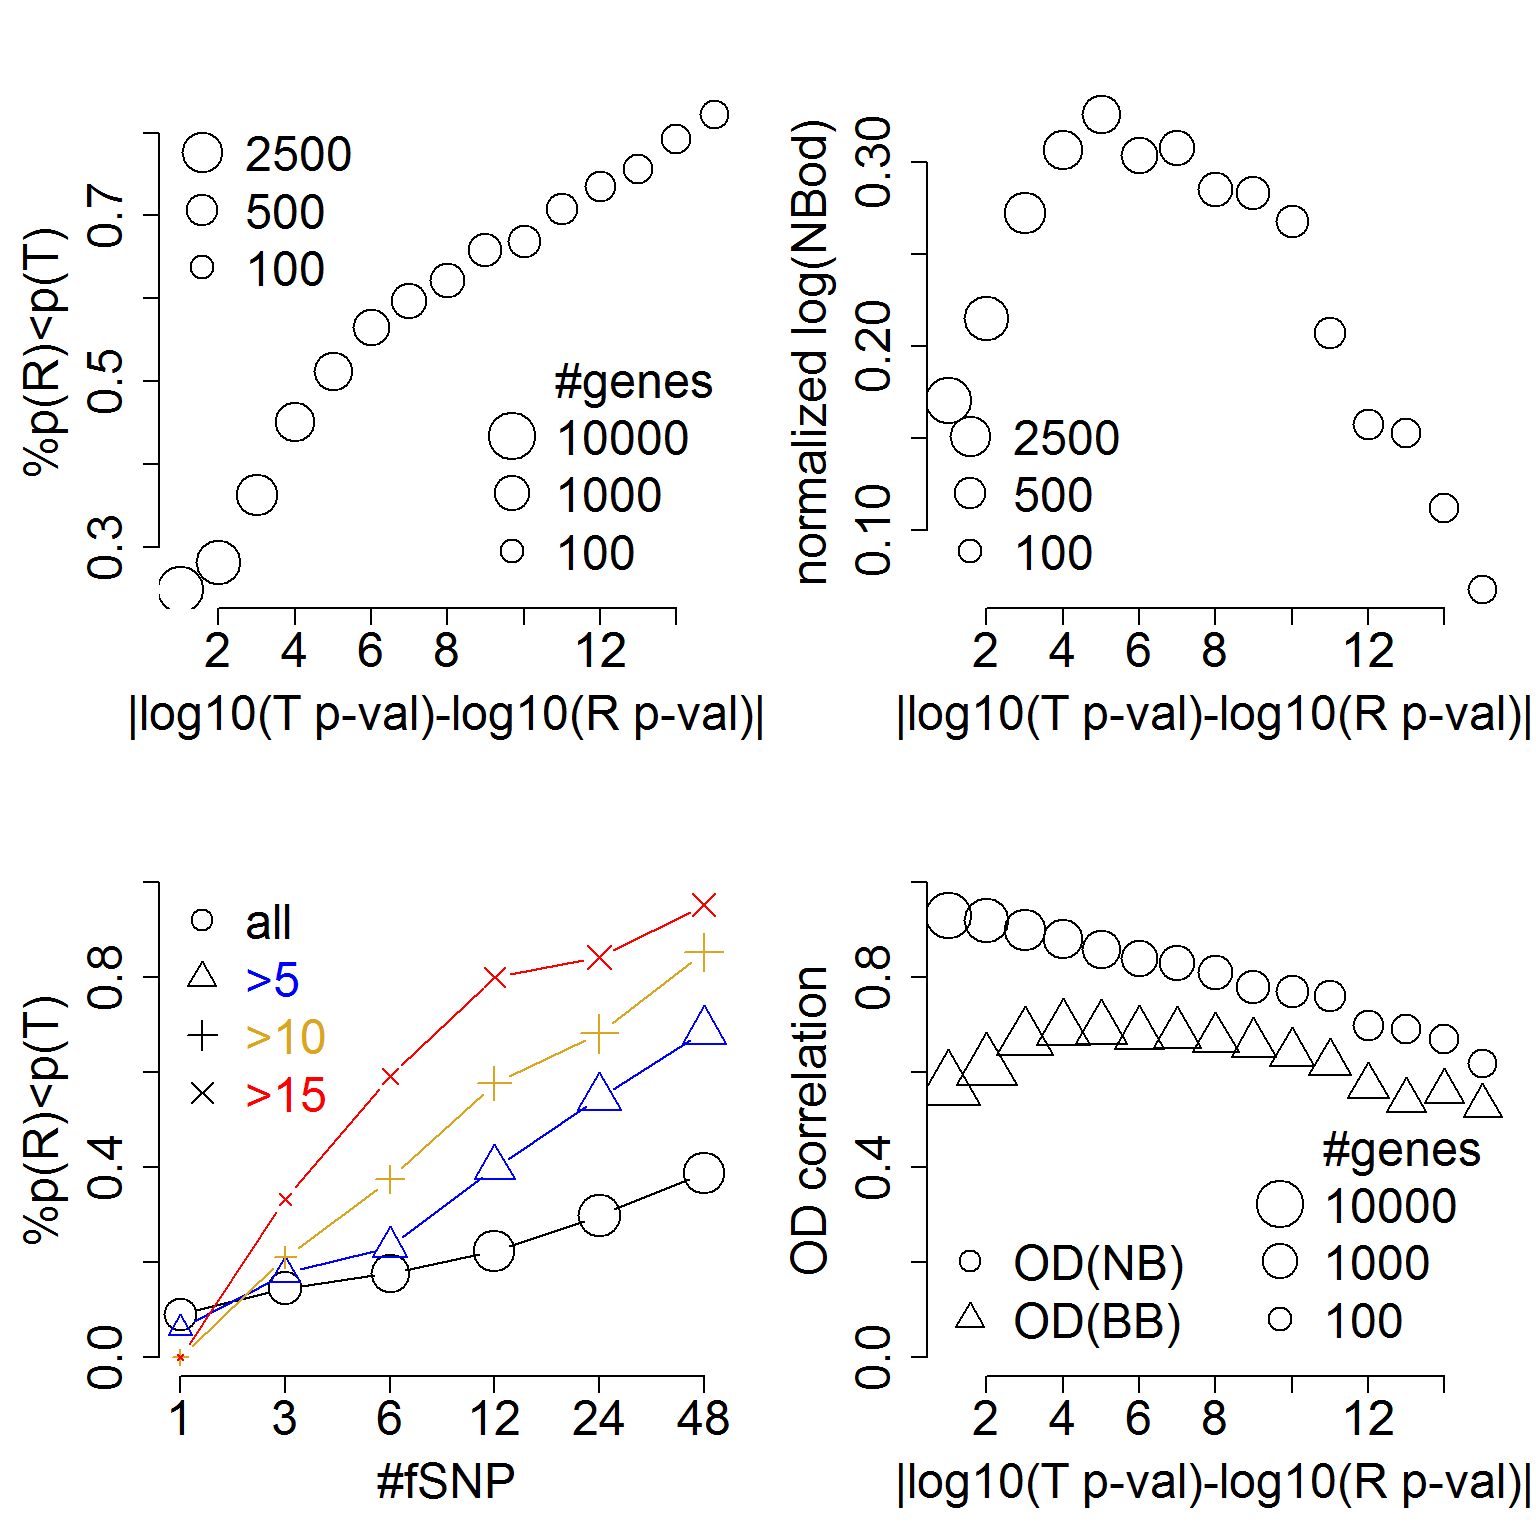
\includegraphics{markdown_files/figure-latex/fig1-1} \end{center}

Plotting Over-dispersions

\begin{Shaded}
\begin{Highlighting}[]
\KeywordTok{par}\NormalTok{(}\DataTypeTok{mfrow=}\KeywordTok{c}\NormalTok{(}\DecValTok{2}\NormalTok{,}\DecValTok{3}\NormalTok{))}
\KeywordTok{par}\NormalTok{(}\DataTypeTok{mar=}\KeywordTok{c}\NormalTok{(}\DecValTok{5}\NormalTok{,}\DecValTok{5}\NormalTok{,}\DecValTok{3}\NormalTok{,}\DecValTok{1}\NormalTok{))}

\KeywordTok{plot}\NormalTok{(}\KeywordTok{density}\NormalTok{(lodNB), }\DataTypeTok{bty=}\StringTok{"n"}\NormalTok{, }\DataTypeTok{main=}\StringTok{"log10(NB OD)"}\NormalTok{, }\DataTypeTok{xlab=}\StringTok{"log(od)"}\NormalTok{, }\DataTypeTok{cex.main=}\NormalTok{cexes, }\DataTypeTok{cex.lab=}\NormalTok{cexes, }\DataTypeTok{cex.axis=}\NormalTok{cexes)}
\KeywordTok{plot}\NormalTok{(}\KeywordTok{density}\NormalTok{(lodBB), }\DataTypeTok{bty=}\StringTok{"n"}\NormalTok{, }\DataTypeTok{main=}\StringTok{"log10(BB OD)"}\NormalTok{, }\DataTypeTok{xlab=}\StringTok{"log(od)"}\NormalTok{, }\DataTypeTok{cex.main=}\NormalTok{cexes, }\DataTypeTok{cex.lab=}\NormalTok{cexes, }\DataTypeTok{cex.axis=}\NormalTok{cexes)}
\KeywordTok{plot}\NormalTok{(}\KeywordTok{density}\NormalTok{(lodR), }\DataTypeTok{bty=}\StringTok{"n"}\NormalTok{, }\DataTypeTok{main=}\StringTok{"log10(RASQ OD)"}\NormalTok{, }\DataTypeTok{xlab=}\StringTok{"log(od)"}\NormalTok{, }\DataTypeTok{cex.main=}\NormalTok{cexes, }\DataTypeTok{cex.lab=}\NormalTok{cexes, }\DataTypeTok{cex.axis=}\NormalTok{cexes)}
\KeywordTok{smoothScatter}\NormalTok{(lodNB, lodBB, }\DataTypeTok{main=}\StringTok{"NB vs BB over-disp"}\NormalTok{, }\DataTypeTok{xlab=}\StringTok{"log(NB OD)"}\NormalTok{, }\DataTypeTok{ylab=}\StringTok{"log(BB OD)"}\NormalTok{, }\DataTypeTok{cex.main=}\NormalTok{cexes, }\DataTypeTok{cex.lab=}\NormalTok{cexes, }\DataTypeTok{cex.axis=}\NormalTok{cexes)}
\KeywordTok{smoothScatter}\NormalTok{(lodNB, lodR, }\DataTypeTok{main=}\StringTok{"NB vs Rasq over-disp"}\NormalTok{, }\DataTypeTok{xlab=}\StringTok{"log(NB OD)"}\NormalTok{, }\DataTypeTok{ylab=}\StringTok{"log(RASQ OD)"}\NormalTok{, }\DataTypeTok{cex.main=}\NormalTok{cexes, }\DataTypeTok{cex.lab=}\NormalTok{cexes, }\DataTypeTok{cex.axis=}\NormalTok{cexes)}
\KeywordTok{smoothScatter}\NormalTok{(lodR, lodBB, }\DataTypeTok{main=}\StringTok{"Rasq vs BB over-disp"}\NormalTok{, }\DataTypeTok{xlab=}\StringTok{"log(RASQ OD)"}\NormalTok{, }\DataTypeTok{ylab=}\StringTok{"log(BB OD)"}\NormalTok{, }\DataTypeTok{cex.main=}\NormalTok{cexes, }\DataTypeTok{cex.lab=}\NormalTok{cexes, }\DataTypeTok{cex.axis=}\NormalTok{cexes)}
\end{Highlighting}
\end{Shaded}

\begin{center}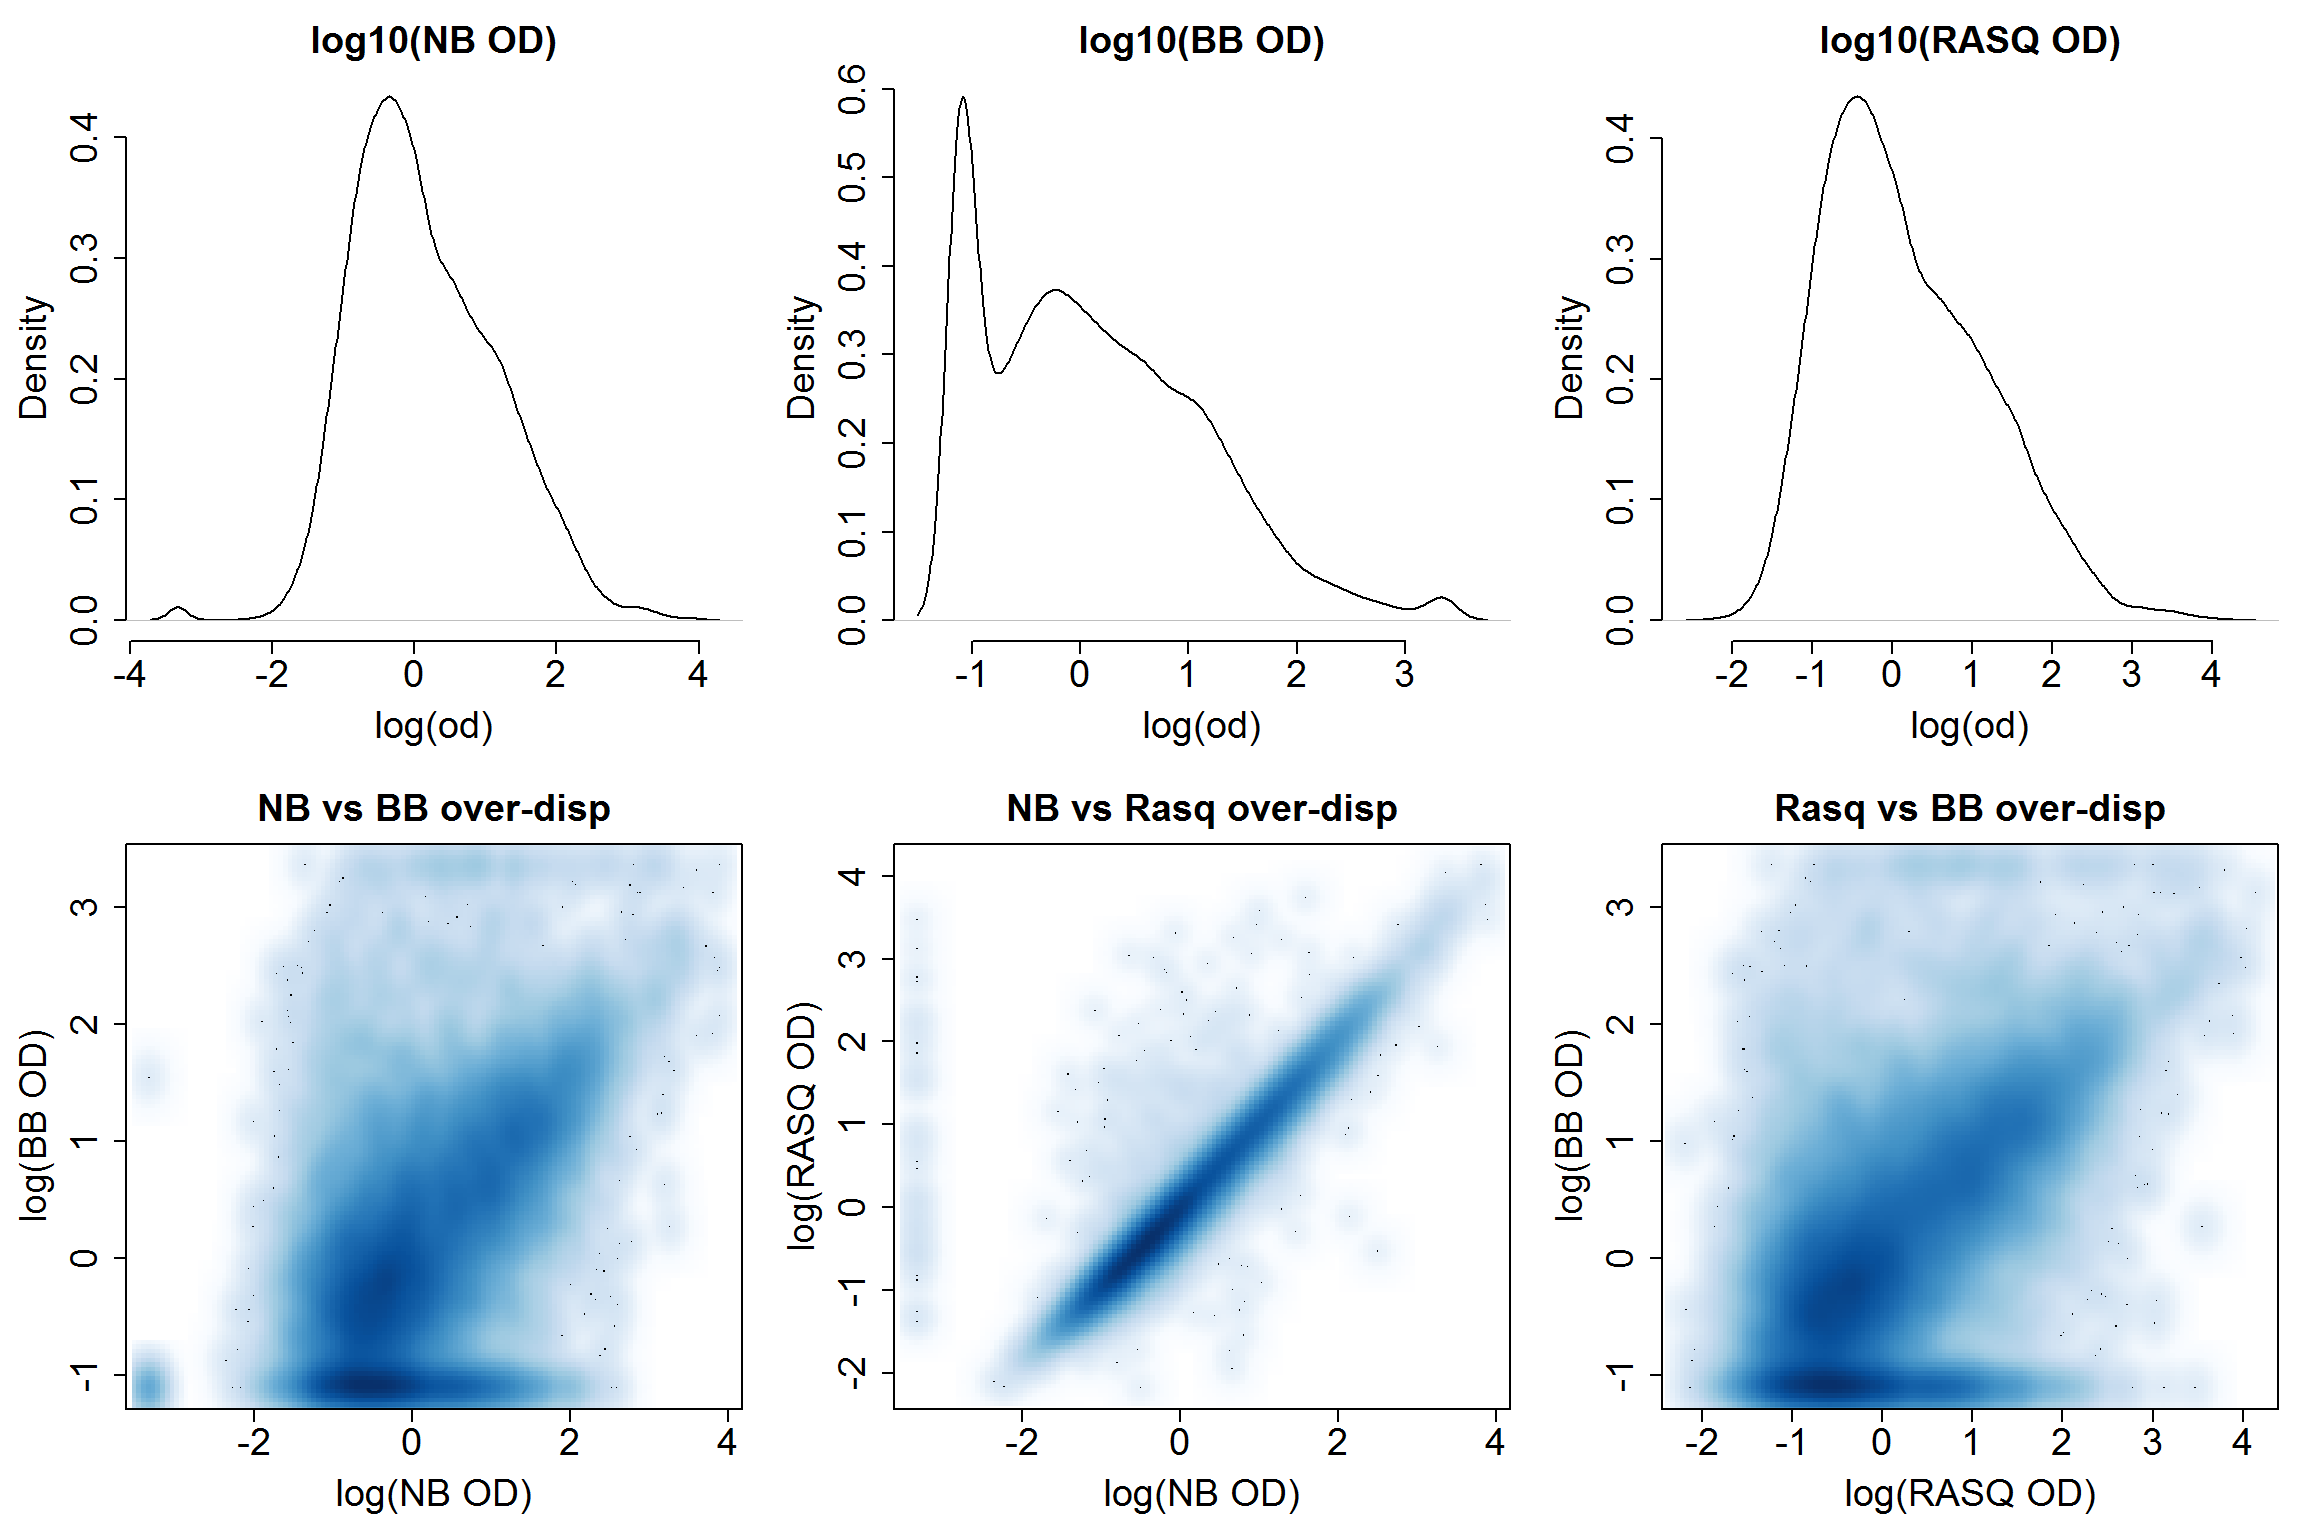
\includegraphics{markdown_files/figure-latex/fig2-1} \end{center}

Plotting RASQUAL read counts, normalized NfSNP and their interaction
along with interactions with BB over-dispersion

\begin{Shaded}
\begin{Highlighting}[]
\KeywordTok{par}\NormalTok{(}\DataTypeTok{mfrow=}\KeywordTok{c}\NormalTok{(}\DecValTok{2}\NormalTok{,}\DecValTok{3}\NormalTok{))}
\KeywordTok{par}\NormalTok{(}\DataTypeTok{mar=}\KeywordTok{c}\NormalTok{(}\DecValTok{5}\NormalTok{,}\DecValTok{5}\NormalTok{,}\DecValTok{3}\NormalTok{,}\DecValTok{1}\NormalTok{))}

\KeywordTok{plot}\NormalTok{(}\KeywordTok{density}\NormalTok{(asR), }\DataTypeTok{bty=}\StringTok{"n"}\NormalTok{, }\DataTypeTok{main=}\StringTok{"#as-RASQ"}\NormalTok{, }\DataTypeTok{xlab=}\StringTok{"#as-RASQUAL"}\NormalTok{, }\DataTypeTok{cex.main=}\NormalTok{cexes, }\DataTypeTok{cex.lab=}\NormalTok{cexes, }\DataTypeTok{cex.axis=}\NormalTok{cexes)}
\KeywordTok{plot}\NormalTok{(}\KeywordTok{density}\NormalTok{(NfSNP), }\DataTypeTok{bty=}\StringTok{"n"}\NormalTok{, }\DataTypeTok{main=}\StringTok{"#fSNPs"}\NormalTok{, }\DataTypeTok{xlab=}\StringTok{"#fSNPs"}\NormalTok{, }\DataTypeTok{cex.main=}\NormalTok{cexes, }\DataTypeTok{cex.lab=}\NormalTok{cexes, }\DataTypeTok{cex.axis=}\NormalTok{cexes)}
\CommentTok{#plot(density(NrSNP), bty="n", main="#rSNPs", xlab="#fSNPs", cex.main=cexes, cex.lab=cexes, cex.axis=cexes)}
\KeywordTok{plot}\NormalTok{(}\KeywordTok{density}\NormalTok{(i12), }\DataTypeTok{bty=}\StringTok{"n"}\NormalTok{, }\DataTypeTok{main=}\StringTok{"interac, #asR & #fSNP"}\NormalTok{, }
     \DataTypeTok{xlab=}\StringTok{"#as-RASQ * #fSNPs"}\NormalTok{, }\DataTypeTok{cex.main=}\NormalTok{cexes, }\DataTypeTok{cex.lab=}\NormalTok{cexes, }\DataTypeTok{cex.axis=}\NormalTok{cexes)}
\KeywordTok{plot}\NormalTok{(}\KeywordTok{density}\NormalTok{(i13), }\DataTypeTok{bty=}\StringTok{"n"}\NormalTok{, }\DataTypeTok{main=}\StringTok{"interac, #asR & #log(BB OD)"}\NormalTok{, }
     \DataTypeTok{xlab=}\StringTok{"#asR * log10(BB OD)"}\NormalTok{, }\DataTypeTok{cex.main=}\NormalTok{cexes, }\DataTypeTok{cex.lab=}\NormalTok{cexes, }\DataTypeTok{cex.axis=}\NormalTok{cexes)}
\KeywordTok{plot}\NormalTok{(}\KeywordTok{density}\NormalTok{(i23), }\DataTypeTok{bty=}\StringTok{"n"}\NormalTok{, }\DataTypeTok{main=}\StringTok{"interac, #fSNP & log(BB OD)"}\NormalTok{, }
     \DataTypeTok{xlab=}\StringTok{"#fSNPs * log10(BB OD)"}\NormalTok{, }\DataTypeTok{cex.main=}\NormalTok{cexes, }\DataTypeTok{cex.lab=}\NormalTok{cexes, }\DataTypeTok{cex.axis=}\NormalTok{cexes)}
\KeywordTok{plot}\NormalTok{(}\KeywordTok{density}\NormalTok{(i123), }\DataTypeTok{bty=}\StringTok{"n"}\NormalTok{, }\DataTypeTok{main=}\StringTok{"interac, #asR & #fSNP & log(BB OD0"}\NormalTok{, }\DataTypeTok{xlim=}\KeywordTok{c}\NormalTok{(}\OperatorTok{-}\DecValTok{10}\NormalTok{,}\DecValTok{10}\NormalTok{),}
     \DataTypeTok{xlab=}\StringTok{"#as-RASQ * #fSNPs * log10(BB OD)"}\NormalTok{, , }\DataTypeTok{cex.main=}\NormalTok{cexes, }\DataTypeTok{cex.lab=}\NormalTok{cexes, }\DataTypeTok{cex.axis=}\NormalTok{cexes)}
\end{Highlighting}
\end{Shaded}

\begin{center}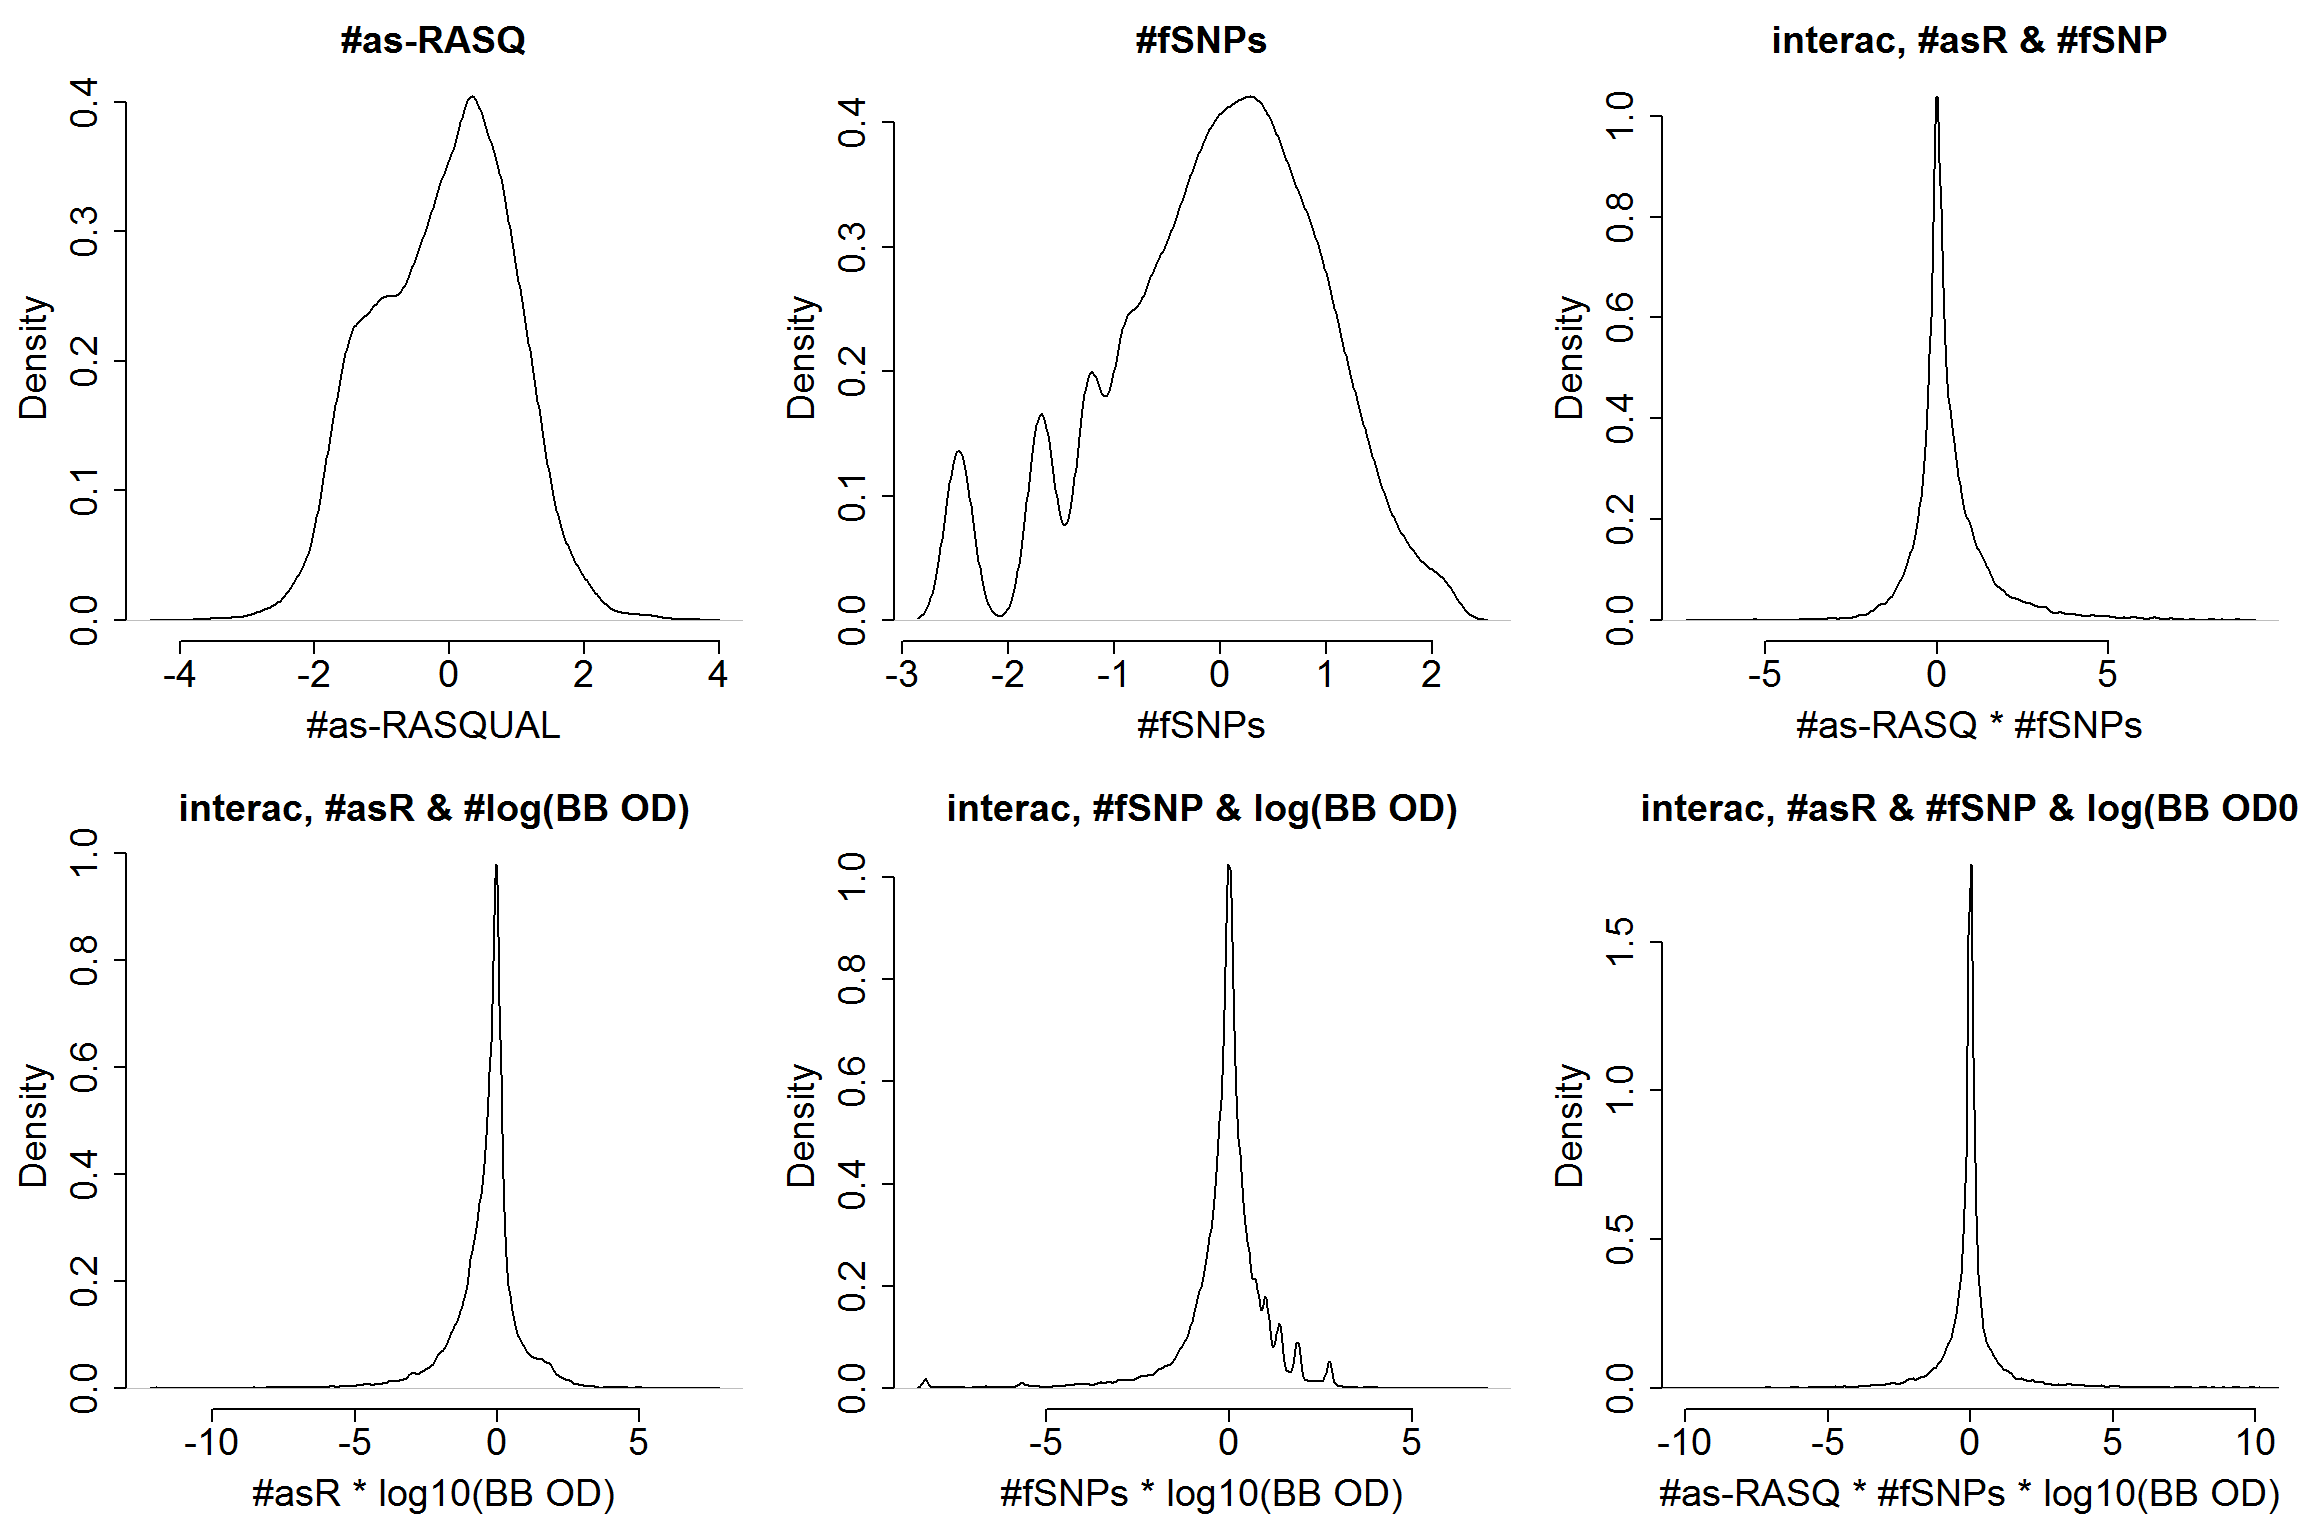
\includegraphics{markdown_files/figure-latex/fig3-1} \end{center}

\begin{Shaded}
\begin{Highlighting}[]
\KeywordTok{par}\NormalTok{(}\DataTypeTok{mfrow=}\KeywordTok{c}\NormalTok{(}\DecValTok{2}\NormalTok{,}\DecValTok{3}\NormalTok{))}
\KeywordTok{par}\NormalTok{(}\DataTypeTok{mar=}\KeywordTok{c}\NormalTok{(}\DecValTok{5}\NormalTok{,}\DecValTok{5}\NormalTok{,}\DecValTok{3}\NormalTok{,}\DecValTok{1}\NormalTok{))}

\KeywordTok{plot}\NormalTok{(}\KeywordTok{density}\NormalTok{(asT), }\DataTypeTok{bty=}\StringTok{"n"}\NormalTok{, }\DataTypeTok{main=}\StringTok{"#as-TReCASE"}\NormalTok{, }
     \DataTypeTok{xlab=}\StringTok{"#as-TReCASE"}\NormalTok{, }\DataTypeTok{cex.main=}\NormalTok{cexes, }\DataTypeTok{cex.lab=}\NormalTok{cexes, }\DataTypeTok{cex.axis=}\NormalTok{cexes)}
\KeywordTok{plot}\NormalTok{(}\KeywordTok{density}\NormalTok{(ia14), }\DataTypeTok{bty=}\StringTok{"n"}\NormalTok{, }\DataTypeTok{main=}\StringTok{"interact, #as-RASQ & #as-TReCASE"}\NormalTok{, }
     \DataTypeTok{xlab=}\StringTok{"#as-RASQ*#as-TReCASE"}\NormalTok{, }\DataTypeTok{cex.main=}\NormalTok{cexes, }\DataTypeTok{cex.lab=}\NormalTok{cexes, }\DataTypeTok{cex.axis=}\NormalTok{cexes)}
\KeywordTok{smoothScatter}\NormalTok{(asT, asR, }\DataTypeTok{bty=}\StringTok{"n"}\NormalTok{, }\DataTypeTok{main=}\StringTok{"#as-RASQ vs #as-TReCASE"}\NormalTok{, }
              \DataTypeTok{xlab=}\StringTok{"#as-TReCASE"}\NormalTok{, }\DataTypeTok{ylab=}\StringTok{"#as-RASQUAL"}\NormalTok{, }\DataTypeTok{cex.main=}\NormalTok{cexes, }\DataTypeTok{cex.lab=}\NormalTok{cexes, }\DataTypeTok{cex.axis=}\NormalTok{cexes)}

\KeywordTok{plot}\NormalTok{(}\KeywordTok{density}\NormalTok{(NrSNP), }\DataTypeTok{bty=}\StringTok{"n"}\NormalTok{, }\DataTypeTok{main=}\StringTok{"#rSNPs"}\NormalTok{, }
     \DataTypeTok{xlab=}\StringTok{"#fSNPs"}\NormalTok{, }\DataTypeTok{cex.main=}\NormalTok{cexes, }\DataTypeTok{cex.lab=}\NormalTok{cexes, }\DataTypeTok{cex.axis=}\NormalTok{cexes)}
\KeywordTok{plot}\NormalTok{(}\KeywordTok{density}\NormalTok{(y), }\DataTypeTok{bty=}\StringTok{"n"}\NormalTok{, }\DataTypeTok{main=}\StringTok{"difference in log10 p-values"}\NormalTok{, }
     \DataTypeTok{xlab=}\StringTok{"log10(T p-val)-log10(R p-val)"}\NormalTok{, }\DataTypeTok{cex.main=}\NormalTok{cexes, }\DataTypeTok{cex.lab=}\NormalTok{cexes, }\DataTypeTok{cex.axis=}\NormalTok{cexes)}
\KeywordTok{smoothScatter}\NormalTok{(rasq}\OperatorTok{$}\NormalTok{tnlt, rasq}\OperatorTok{$}\NormalTok{rnlt, }\DataTypeTok{bty=}\StringTok{"n"}\NormalTok{, }\DataTypeTok{main=}\StringTok{"RASQUAL vs TReCASE p-val"}\NormalTok{, }
              \DataTypeTok{xlab=}\StringTok{"-log10(T p-val)"}\NormalTok{, }\DataTypeTok{ylab=}\StringTok{"-log10(R p-val)"}\NormalTok{, }\DataTypeTok{cex.main=}\NormalTok{cexes, }\DataTypeTok{cex.lab=}\NormalTok{cexes, }\DataTypeTok{cex.axis=}\NormalTok{cexes)}
\end{Highlighting}
\end{Shaded}

\begin{center}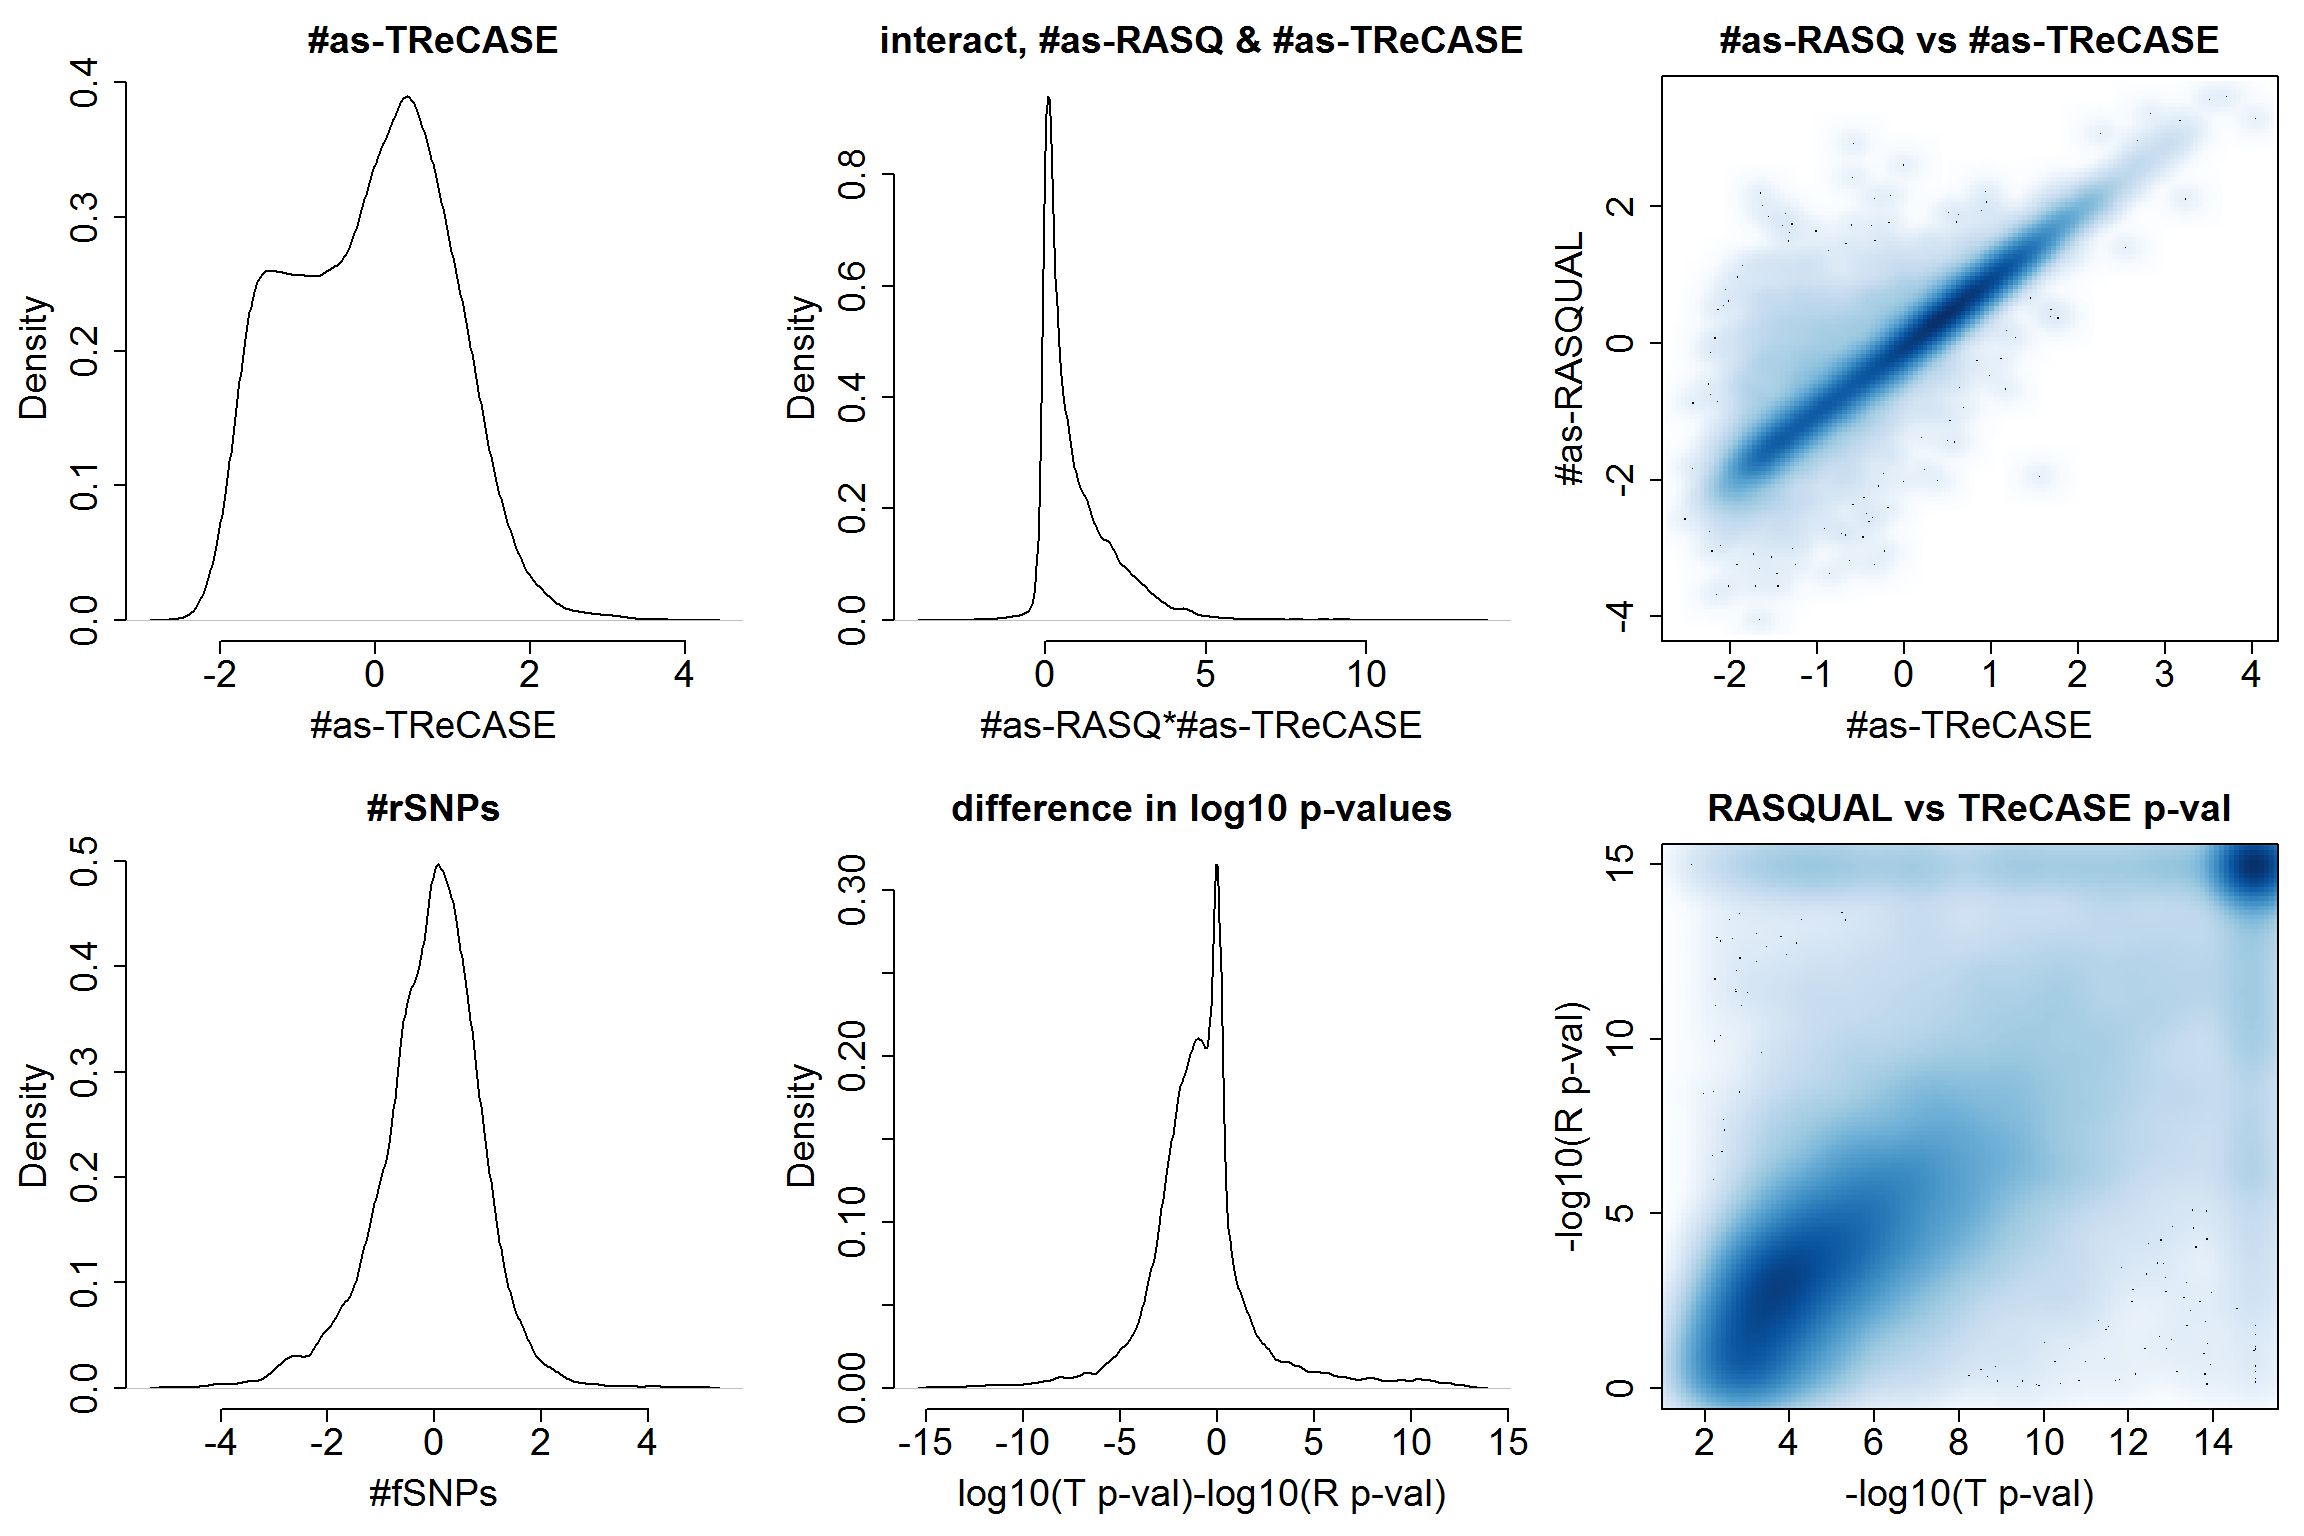
\includegraphics{markdown_files/figure-latex/fig4-1} \end{center}

\begin{Shaded}
\begin{Highlighting}[]
\CommentTok{#rasq$rnlt-rasq$tnlt") - negative implies TReCASE is more significant}
\end{Highlighting}
\end{Shaded}

Other covariates: median permuted p-value, mapping error, reference bias
and Chi2 of Hardy Weinberg Equilibrium

\begin{Shaded}
\begin{Highlighting}[]
\KeywordTok{par}\NormalTok{(}\DataTypeTok{mfrow=}\KeywordTok{c}\NormalTok{(}\DecValTok{2}\NormalTok{,}\DecValTok{2}\NormalTok{))}
\KeywordTok{par}\NormalTok{(}\DataTypeTok{mar=}\KeywordTok{c}\NormalTok{(}\DecValTok{5}\NormalTok{,}\DecValTok{5}\NormalTok{,}\DecValTok{3}\NormalTok{,}\DecValTok{1}\NormalTok{))}
\KeywordTok{plot}\NormalTok{(}\KeywordTok{density}\NormalTok{(mpp), }\DataTypeTok{bty=}\StringTok{"n"}\NormalTok{, }\DataTypeTok{main=}\StringTok{"#median permuted p-val"}\NormalTok{, }
     \DataTypeTok{xlab=}\StringTok{"normalized p-value"}\NormalTok{, }\DataTypeTok{cex.main=}\NormalTok{cexes, }\DataTypeTok{cex.lab=}\NormalTok{cexes, }\DataTypeTok{cex.axis=}\NormalTok{cexes)}
\KeywordTok{plot}\NormalTok{(}\KeywordTok{density}\NormalTok{(derr), }\DataTypeTok{bty=}\StringTok{"n"}\NormalTok{, }\DataTypeTok{main=}\StringTok{"mapping error"}\NormalTok{, }
     \DataTypeTok{xlab=}\StringTok{"normalized error"}\NormalTok{, }\DataTypeTok{cex.main=}\NormalTok{cexes, }\DataTypeTok{cex.lab=}\NormalTok{cexes, }\DataTypeTok{cex.axis=}\NormalTok{cexes)}
\KeywordTok{plot}\NormalTok{(}\KeywordTok{density}\NormalTok{(phib), }\DataTypeTok{bty=}\StringTok{"n"}\NormalTok{, }\DataTypeTok{main=}\StringTok{"#reference bias"}\NormalTok{, }
     \DataTypeTok{xlab=}\StringTok{"normalized deviation from 0.5"}\NormalTok{, }\DataTypeTok{cex.main=}\NormalTok{cexes, }\DataTypeTok{cex.lab=}\NormalTok{cexes, }\DataTypeTok{cex.axis=}\NormalTok{cexes)}
\KeywordTok{plot}\NormalTok{(}\KeywordTok{density}\NormalTok{(hwec2), }\DataTypeTok{bty=}\StringTok{"n"}\NormalTok{, }\DataTypeTok{main=}\StringTok{"#HWE equilibrium"}\NormalTok{, }
     \DataTypeTok{xlab=}\StringTok{"log(Chi2)"}\NormalTok{, }\DataTypeTok{cex.main=}\NormalTok{cexes, }\DataTypeTok{cex.lab=}\NormalTok{cexes, }\DataTypeTok{cex.axis=}\NormalTok{cexes)}
\end{Highlighting}
\end{Shaded}

\begin{center}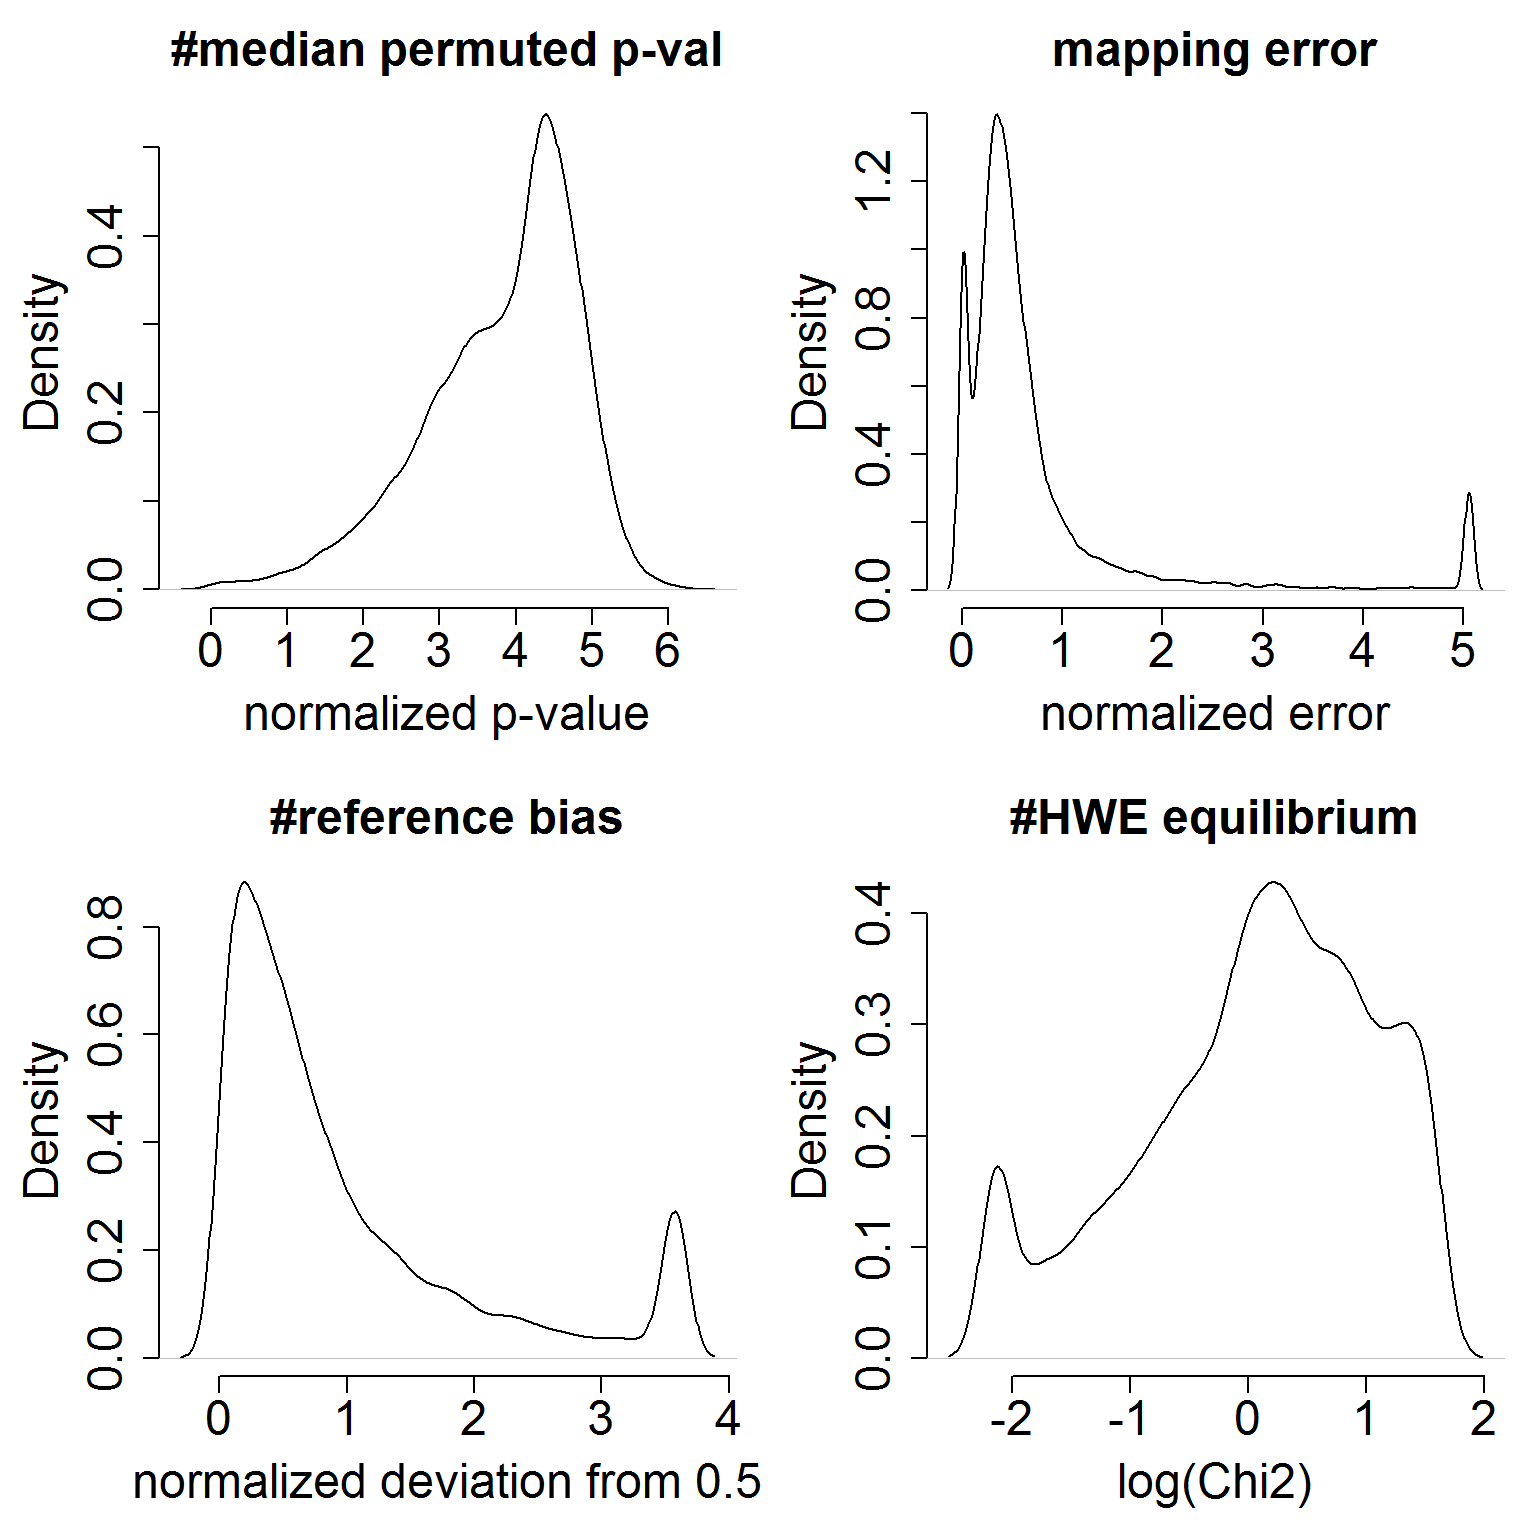
\includegraphics{markdown_files/figure-latex/fig5-1} \end{center}

Fitting all 13978 genes

\begin{Shaded}
\begin{Highlighting}[]
\CommentTok{#with several cutoffs}
\CommentTok{#kp = abs(y)>=(cutoff-5)}
\NormalTok{cutsub =}\StringTok{ }\DecValTok{0}
\NormalTok{kp =}\StringTok{ }\KeywordTok{abs}\NormalTok{(y)}\OperatorTok{>=}\NormalTok{cutsub}
\KeywordTok{sum}\NormalTok{(kp)}
\end{Highlighting}
\end{Shaded}

\begin{verbatim}
## [1] 13978
\end{verbatim}

\begin{Shaded}
\begin{Highlighting}[]
\NormalTok{resA =}\StringTok{ }\KeywordTok{subset_fit}\NormalTok{(kp, }\DataTypeTok{digits=}\DecValTok{3}\NormalTok{)}
\end{Highlighting}
\end{Shaded}

\begin{verbatim}
## Loading required package: carData
\end{verbatim}

\begin{Shaded}
\begin{Highlighting}[]
\NormalTok{resA}\OperatorTok{$}\NormalTok{tab}
\end{Highlighting}
\end{Shaded}

\begin{verbatim}
##                           Est      SE      P-val      Marg.Est Marg.P    
## (Intercept)               "-0.611" "0.156" " 9.1e-05" "-0.825" "4.8e-242"
## log(OD_BB)                "0.891"  "0.031" "1.1e-172" "0.33"   " 4.0e-42"
## ASReC_R                   "0.868"  "0.069" " 3.9e-36" "0.434"  " 6.9e-72"
## n-fSNP                    "0.465"  "0.03"  " 2.1e-55" "0.495"  " 3.2e-93"
## ASReC_R:n-SNP             "0.256"  "0.026" " 3.9e-22" "0.024"  " 2.6e-01"
## ASReC_R:log(OD_BB)        "0.567"  "0.026" "6.9e-105" "0.38"   " 2.5e-75"
## n-fSNP:log(OD_BB)         "0.319"  "0.025" " 1.8e-36" "0.191"  " 1.3e-20"
## ASReC_R:n-fSNP:log(OD_BB) "0.167"  "0.019" " 1.2e-18" "-0.073" " 2.0e-07"
## n-rSNP                    "0.049"  "0.025" " 4.6e-02" "0.26"   " 2.1e-26"
## log(OD_NB)                "-0.417" "0.031" " 2.4e-42" "-0.156" " 1.5e-10"
## ASReC_T                   "-0.547" "0.064" " 1.1e-17" "0.321"  " 7.2e-40"
## ASReC_T:ASReC_R           "0.117"  "0.022" " 8.4e-08" "-0.049" " 1.8e-02"
## AF                        "0.005"  "0.022" " 8.3e-01" "0.013"  " 6.0e-01"
## Chi2-HWEC                 "-0.119" "0.023" " 1.4e-07" "-0.149" " 9.3e-10"
## Map.Err                   "-0.119" "0.027" " 1.2e-05" "0.1"    " 4.1e-05"
## Ref.Bias                  "0.248"  "0.028" " 3.0e-18" "0.204"  " 4.4e-17"
## Med(perm-p)               "-0.089" "0.038" " 1.9e-02" "-0.392" " 6.6e-59"
\end{verbatim}

\begin{Shaded}
\begin{Highlighting}[]
\NormalTok{resA}\OperatorTok{$}\NormalTok{ano}
\end{Highlighting}
\end{Shaded}

\begin{verbatim}
##                           SumSq Typ1per  T1P-val Typ3per  T3P-val Marg.R
## log(OD_BB)                 1521     1.3  1.7e-48     4.9 1.1e-172    1.3
## ASReC_R                    4760     4.1 1.7e-145       1  3.9e-36    2.3
## n-fSNP                     1685     1.5  1.7e-53     1.5  2.1e-55    3.0
## ASReC_R:n-SNP               828     0.7  2.8e-27     0.6  3.9e-22    0.0
## ASReC_R:log(OD_BB)         4718     4.1 3.1e-144     2.9 6.9e-105    2.4
## n-fSNP:log(OD_BB)           732     0.6  2.6e-24       1  1.8e-36    0.6
## ASReC_R:n-fSNP:log(OD_BB)   474     0.4  2.6e-16     0.5  1.2e-18    0.2
## n-rSNP                        1     0.0  7.7e-01       0  4.6e-02    0.8
## log(OD_NB)                 1051     0.9  3.8e-34     1.1  2.4e-42    0.3
## ASReC_T                     472     0.4  2.9e-16     0.4  1.1e-17    1.2
## ASReC_T:ASReC_R             267     0.2  7.9e-10     0.2  8.4e-08    0.0
## AF                            1     0.0  6.7e-01       0  8.3e-01    0.0
## Chi2-HWEC                   207     0.2  6.0e-08     0.2  1.4e-07    0.3
## Map.Err                      10     0.0  2.4e-01     0.1  1.2e-05    0.1
## Ref.Bias                    538     0.5  2.7e-18     0.5  3.0e-18    0.5
## Med(perm-p)                  39     0.0  1.9e-02       0  1.9e-02    1.9
\end{verbatim}

\begin{Shaded}
\begin{Highlighting}[]
\NormalTok{resA}\OperatorTok{$}\NormalTok{r2}
\end{Highlighting}
\end{Shaded}

\begin{verbatim}
## [1] 0.1495812
\end{verbatim}

\begin{Shaded}
\begin{Highlighting}[]
\KeywordTok{write.csv}\NormalTok{(resA}\OperatorTok{$}\NormalTok{ano, }\KeywordTok{sprintf}\NormalTok{(}\StringTok{"anova_cut%s.csv"}\NormalTok{, cutsub), }\DataTypeTok{quote=}\NormalTok{F)}
\KeywordTok{write.csv}\NormalTok{(resA}\OperatorTok{$}\NormalTok{tab, }\KeywordTok{sprintf}\NormalTok{(}\StringTok{"model_cut%s.csv"}\NormalTok{, cutsub), }\DataTypeTok{quote=}\NormalTok{F)}
\end{Highlighting}
\end{Shaded}

Less stringent cutoff (1204 genes)

\begin{Shaded}
\begin{Highlighting}[]
\NormalTok{cutsub =}\StringTok{ }\DecValTok{5}
\NormalTok{kp =}\StringTok{ }\KeywordTok{abs}\NormalTok{(y)}\OperatorTok{>=}\NormalTok{cutsub}
\KeywordTok{sum}\NormalTok{(kp)}
\end{Highlighting}
\end{Shaded}

\begin{verbatim}
## [1] 1204
\end{verbatim}

\begin{Shaded}
\begin{Highlighting}[]
\NormalTok{resA =}\StringTok{ }\KeywordTok{subset_fit}\NormalTok{(kp)}

\NormalTok{resA}\OperatorTok{$}\NormalTok{tab}
\end{Highlighting}
\end{Shaded}

\begin{verbatim}
##                           Est      SE      P-val     Marg.Est Marg.P   
## (Intercept)               "-2.403" "1.097" "2.9e-02" "-0.071" "7.6e-01"
## log(OD_BB)                "2.873"  "0.226" "8.8e-35" "1.284"  "1.6e-10"
## ASReC_R                   "3.215"  "0.482" "3.9e-11" "2.293"  "2.7e-26"
## n-fSNP                    "1.758"  "0.286" "1.0e-09" "2.542"  "8.7e-28"
## ASReC_R:n-SNP             "0.711"  "0.243" "3.6e-03" "0.676"  "1.0e-03"
## ASReC_R:log(OD_BB)        "1.159"  "0.181" "2.1e-10" "2.415"  "6.9e-54"
## n-fSNP:log(OD_BB)         "0.343"  "0.179" "5.6e-02" "1.009"  "1.3e-09"
## ASReC_R:n-fSNP:log(OD_BB) "0.12"   "0.146" "4.1e-01" "-0.352" "6.5e-03"
## n-rSNP                    "-0.093" "0.202" "6.4e-01" "0.554"  "2.1e-02"
## log(OD_NB)                "-2.091" "0.224" "5.3e-20" "-1.829" "1.6e-19"
## ASReC_T                   "-1.536" "0.433" "4.0e-04" "1.651"  "5.3e-15"
## ASReC_T:ASReC_R           "-0.169" "0.146" "2.5e-01" "-0.478" "2.4e-03"
## AF                        "-0.312" "0.177" "7.8e-02" "-0.613" "7.0e-03"
## Chi2-HWEC                 "-0.403" "0.184" "2.9e-02" "-0.334" "1.6e-01"
## Map.Err                   "-0.409" "0.17"  "1.6e-02" "0.24"   "1.5e-01"
## Ref.Bias                  "0.914"  "0.192" "2.2e-06" "0.963"  "3.1e-07"
## Med(perm-p)               "0.246"  "0.272" "3.7e-01" "-1.534" "8.5e-15"
\end{verbatim}

\begin{Shaded}
\begin{Highlighting}[]
\NormalTok{resA}\OperatorTok{$}\NormalTok{ano}
\end{Highlighting}
\end{Shaded}

\begin{verbatim}
##                           SumSq Typ1per T1P-val Typ3per T3P-val Marg.R
## log(OD_BB)                 2576     3.3 4.6e-16       8 8.8e-35    3.3
## ASReC_R                   13286    17.2 1.2e-68     2.2 3.9e-11    8.9
## n-fSNP                     5045     6.5 3.2e-29     1.9 1.0e-09    9.5
## ASReC_R:n-SNP               130     0.2 6.5e-02     0.4 3.6e-03    0.9
## ASReC_R:log(OD_BB)         4444     5.8 4.4e-26       2 2.1e-10   18.0
## n-fSNP:log(OD_BB)           360     0.5 2.1e-03     0.2 5.6e-02    3.0
## ASReC_R:n-fSNP:log(OD_BB)   168     0.2 3.5e-02       0 4.1e-01    0.6
## n-rSNP                      285     0.4 6.2e-03       0 6.4e-01    0.4
## log(OD_NB)                 3698     4.8 3.9e-22     4.3 5.3e-20    6.6
## ASReC_T                     738     1.0 1.1e-05     0.6 4.0e-04    5.0
## ASReC_T:ASReC_R              58     0.1 2.2e-01     0.1 2.5e-01    0.8
## AF                           84     0.1 1.4e-01     0.2 7.8e-02    0.6
## Chi2-HWEC                   227     0.3 1.5e-02     0.2 2.9e-02    0.2
## Map.Err                       2     0.0 8.2e-01     0.3 1.6e-02    0.2
## Ref.Bias                    877     1.1 1.7e-06     1.1 2.2e-06    2.2
## Med(perm-p)                  31     0.0 3.7e-01       0 3.7e-01    4.9
\end{verbatim}

\begin{Shaded}
\begin{Highlighting}[]
\NormalTok{resA}\OperatorTok{$}\NormalTok{r2}
\end{Highlighting}
\end{Shaded}

\begin{verbatim}
## [1] 0.4153098
\end{verbatim}

\begin{Shaded}
\begin{Highlighting}[]
\KeywordTok{write.csv}\NormalTok{(resA}\OperatorTok{$}\NormalTok{ano, }\KeywordTok{sprintf}\NormalTok{(}\StringTok{"anova_cut%s.csv"}\NormalTok{, cutsub), }\DataTypeTok{quote=}\NormalTok{F)}
\KeywordTok{write.csv}\NormalTok{(resA}\OperatorTok{$}\NormalTok{tab, }\KeywordTok{sprintf}\NormalTok{(}\StringTok{"model_cut%s.csv"}\NormalTok{, cutsub), }\DataTypeTok{quote=}\NormalTok{F)}
\end{Highlighting}
\end{Shaded}

The most discrepant 221 genes

\begin{Shaded}
\begin{Highlighting}[]
\NormalTok{cutsub =}\StringTok{ }\NormalTok{cutoff}\OperatorTok{-}\DecValTok{5}
\NormalTok{kp =}\StringTok{ }\KeywordTok{abs}\NormalTok{(y)}\OperatorTok{>=}\NormalTok{cutsub}
\KeywordTok{sum}\NormalTok{(kp)}
\end{Highlighting}
\end{Shaded}

\begin{verbatim}
## [1] 221
\end{verbatim}

\begin{Shaded}
\begin{Highlighting}[]
\NormalTok{resA =}\StringTok{ }\KeywordTok{subset_fit}\NormalTok{(kp)}

\NormalTok{resA}\OperatorTok{$}\NormalTok{tab}
\end{Highlighting}
\end{Shaded}

\begin{verbatim}
##                           Est      SE      P-val     Marg.Est Marg.P   
## (Intercept)               "5.493"  "3.357" "1.0e-01" "3.475"  "4.1e-06"
## log(OD_BB)                "3.51"   "0.624" "6.1e-08" "0.126"  "8.4e-01"
## ASReC_R                   "2.991"  "1.389" "3.2e-02" "4.531"  "1.8e-09"
## n-fSNP                    "2.903"  "1.164" "1.3e-02" "5.071"  "5.9e-12"
## ASReC_R:n-SNP             "0.753"  "0.979" "4.4e-01" "0.351"  "6.4e-01"
## ASReC_R:log(OD_BB)        "0.472"  "0.588" "4.2e-01" "3.679"  "3.3e-18"
## n-fSNP:log(OD_BB)         "0.197"  "0.559" "7.2e-01" "2.147"  "1.5e-07"
## ASReC_R:n-fSNP:log(OD_BB) "-0.506" "0.485" "3.0e-01" "-1.656" "2.3e-05"
## n-rSNP                    "-0.185" "0.554" "7.4e-01" "0.162"  "8.3e-01"
## log(OD_NB)                "-3.269" "0.577" "4.9e-08" "-4.463" "5.1e-16"
## ASReC_T                   "-0.576" "1.064" "5.9e-01" "3.406"  "2.1e-06"
## ASReC_T:ASReC_R           "-1.545" "0.455" "8.2e-04" "-1.78"  "1.3e-03"
## AF                        "-0.698" "0.51"  "1.7e-01" "-1.437" "4.0e-02"
## Chi2-HWEC                 "-0.102" "0.585" "8.6e-01" "0.618"  "4.5e-01"
## Map.Err                   "-0.515" "0.42"  "2.2e-01" "-1.086" "1.1e-02"
## Ref.Bias                  "1.291"  "0.501" "1.1e-02" "0.092"  "8.7e-01"
## Med(perm-p)               "-1.175" "0.831" "1.6e-01" "-3.696" "1.6e-08"
\end{verbatim}

\begin{Shaded}
\begin{Highlighting}[]
\NormalTok{resA}\OperatorTok{$}\NormalTok{ano}
\end{Highlighting}
\end{Shaded}

\begin{verbatim}
##                           SumSq Typ1per T1P-val Typ3per T3P-val Marg.R
## log(OD_BB)                    5     0.0 7.6e-01     6.6 6.1e-08    0.0
## ASReC_R                    5142    19.6 1.8e-18       1 3.2e-02   15.3
## n-fSNP                     4021    15.3 2.8e-15     1.3 1.3e-02   19.5
## ASReC_R:n-SNP                92     0.3 2.0e-01     0.1 4.4e-01    0.1
## ASReC_R:log(OD_BB)         1522     5.8 3.5e-07     0.1 4.2e-01   29.3
## n-fSNP:log(OD_BB)            71     0.3 2.6e-01       0 7.2e-01   11.9
## ASReC_R:n-fSNP:log(OD_BB)     0     0.0 9.6e-01     0.2 3.0e-01    7.9
## n-rSNP                      234     0.9 4.0e-02       0 7.4e-01    0.0
## log(OD_NB)                 2554     9.7 1.0e-10     6.7 4.9e-08   26.0
## ASReC_T                     157     0.6 9.2e-02     0.1 5.9e-01    9.8
## ASReC_T:ASReC_R             817     3.1 1.5e-04     2.4 8.2e-04    4.6
## AF                           35     0.1 4.3e-01     0.4 1.7e-01    1.9
## Chi2-HWEC                    11     0.0 6.5e-01       0 8.6e-01    0.3
## Map.Err                       2     0.0 8.6e-01     0.3 2.2e-01    2.9
## Ref.Bias                    324     1.2 1.6e-02     1.4 1.1e-02    0.0
## Med(perm-p)                 110     0.4 1.6e-01     0.4 1.6e-01   13.6
\end{verbatim}

\begin{Shaded}
\begin{Highlighting}[]
\NormalTok{resA}\OperatorTok{$}\NormalTok{r2}
\end{Highlighting}
\end{Shaded}

\begin{verbatim}
## [1] 0.5740302
\end{verbatim}

\begin{Shaded}
\begin{Highlighting}[]
\KeywordTok{write.csv}\NormalTok{(resA}\OperatorTok{$}\NormalTok{ano, }\KeywordTok{sprintf}\NormalTok{(}\StringTok{"anova_cut%s.csv"}\NormalTok{, cutsub), }\DataTypeTok{quote=}\NormalTok{F)}
\KeywordTok{write.csv}\NormalTok{(resA}\OperatorTok{$}\NormalTok{tab, }\KeywordTok{sprintf}\NormalTok{(}\StringTok{"model_cut%s.csv"}\NormalTok{, cutsub), }\DataTypeTok{quote=}\NormalTok{F)}
\end{Highlighting}
\end{Shaded}

Keeping only genes with difference \textless{}10

\begin{Shaded}
\begin{Highlighting}[]
\NormalTok{cutsub =}\StringTok{ }\DecValTok{10}
\NormalTok{kp =}\StringTok{ }\KeywordTok{abs}\NormalTok{(y)}\OperatorTok{<}\NormalTok{cutsub}
\KeywordTok{sum}\NormalTok{(kp)}
\end{Highlighting}
\end{Shaded}

\begin{verbatim}
## [1] 13757
\end{verbatim}

\begin{Shaded}
\begin{Highlighting}[]
\NormalTok{resA =}\StringTok{ }\KeywordTok{subset_fit}\NormalTok{(kp)}

\NormalTok{resA}\OperatorTok{$}\NormalTok{tab}
\end{Highlighting}
\end{Shaded}

\begin{verbatim}
##                           Est      SE      P-val      Marg.Est Marg.P   
## (Intercept)               "-0.842" "0.138" " 1.1e-09" "-0.894" "0.0e+00"
## log(OD_BB)                "0.703"  "0.028" "3.9e-135" "0.276"  "5.0e-38"
## ASReC_R                   "0.774"  "0.061" " 2.8e-36" "0.343"  "2.5e-59"
## n-fSNP                    "0.399"  "0.026" " 3.4e-52" "0.427"  "1.9e-91"
## ASReC_R:n-SNP             "0.222"  "0.023" " 2.3e-21" "0.026"  "1.6e-01"
## ASReC_R:log(OD_BB)        "0.439"  "0.023" " 1.1e-79" "0.266"  "3.4e-48"
## n-fSNP:log(OD_BB)         "0.244"  "0.023" " 3.9e-27" "0.136"  "6.1e-14"
## ASReC_R:n-fSNP:log(OD_BB) "0.134"  "0.017" " 1.7e-15" "-0.052" "2.4e-05"
## n-rSNP                    "0.072"  "0.022" " 9.2e-04" "0.262"  "9.3e-35"
## log(OD_NB)                "-0.286" "0.027" " 8.2e-26" "-0.065" "2.3e-03"
## ASReC_T                   "-0.484" "0.057" " 1.8e-17" "0.246"  "4.3e-31"
## ASReC_T:ASReC_R           "0.114"  "0.019" " 3.8e-09" "-0.012" "4.9e-01"
## AF                        "0.03"   "0.02"  " 1.3e-01" "0.044"  "3.9e-02"
## Chi2-HWEC                 "-0.132" "0.02"  " 3.7e-11" "-0.168" "2.4e-15"
## Map.Err                   "-0.082" "0.024" " 7.2e-04" "0.09"   "3.2e-05"
## Ref.Bias                  "0.173"  "0.025" " 1.0e-11" "0.145"  "1.8e-11"
## Med(perm-p)               "-0.048" "0.034" " 1.5e-01" "-0.317" "7.9e-51"
\end{verbatim}

\begin{Shaded}
\begin{Highlighting}[]
\NormalTok{resA}\OperatorTok{$}\NormalTok{ano}
\end{Highlighting}
\end{Shaded}

\begin{verbatim}
##                           SumSq Typ1per  T1P-val Typ3per  T3P-val Marg.R
## log(OD_BB)                 1024     1.2  9.8e-43       4 3.9e-135    1.2
## ASReC_R                    3037     3.6 1.4e-121       1  2.8e-36    1.9
## n-fSNP                     1315     1.5  2.8e-54     1.5  3.4e-52    2.9
## ASReC_R:n-SNP               619     0.7  1.4e-26     0.6  2.3e-21    0.0
## ASReC_R:log(OD_BB)         2601     3.1 1.0e-104     2.3  1.1e-79    1.5
## n-fSNP:log(OD_BB)           414     0.5  2.6e-18     0.7  3.9e-27    0.4
## ASReC_R:n-fSNP:log(OD_BB)   279     0.3  7.7e-13     0.4  1.7e-15    0.1
## n-rSNP                       30     0.0  1.8e-02     0.1  9.2e-04    1.1
## log(OD_NB)                  400     0.5  9.5e-18     0.7  8.2e-26    0.1
## ASReC_T                     353     0.4  7.1e-16     0.5  1.8e-17    1.0
## ASReC_T:ASReC_R             233     0.3  5.3e-11     0.2  3.8e-09    0.0
## AF                           15     0.0  9.6e-02       0  1.3e-01    0.0
## Chi2-HWEC                   246     0.3  1.7e-11     0.3  3.7e-11    0.5
## Map.Err                       5     0.0  3.6e-01     0.1  7.2e-04    0.1
## Ref.Bias                    252     0.3  9.5e-12     0.3  1.0e-11    0.3
## Med(perm-p)                  11     0.0  1.5e-01       0  1.5e-01    1.6
\end{verbatim}

\begin{Shaded}
\begin{Highlighting}[]
\NormalTok{resA}\OperatorTok{$}\NormalTok{r2}
\end{Highlighting}
\end{Shaded}

\begin{verbatim}
## [1] 0.1271158
\end{verbatim}

\begin{Shaded}
\begin{Highlighting}[]
\KeywordTok{write.csv}\NormalTok{(resA}\OperatorTok{$}\NormalTok{ano, }\KeywordTok{sprintf}\NormalTok{(}\StringTok{"anova_less%s.csv"}\NormalTok{, cutsub), }\DataTypeTok{quote=}\NormalTok{F)}
\KeywordTok{write.csv}\NormalTok{(resA}\OperatorTok{$}\NormalTok{tab, }\KeywordTok{sprintf}\NormalTok{(}\StringTok{"model_less%s.csv"}\NormalTok{, cutsub), }\DataTypeTok{quote=}\NormalTok{F)}
\end{Highlighting}
\end{Shaded}

Keeping only genes with difference \textless{}5

\begin{Shaded}
\begin{Highlighting}[]
\NormalTok{cutsub =}\StringTok{ }\DecValTok{5}
\NormalTok{kp =}\StringTok{ }\KeywordTok{abs}\NormalTok{(y)}\OperatorTok{<}\NormalTok{cutsub}
\KeywordTok{sum}\NormalTok{(kp)}
\end{Highlighting}
\end{Shaded}

\begin{verbatim}
## [1] 12774
\end{verbatim}

\begin{Shaded}
\begin{Highlighting}[]
\NormalTok{resA =}\StringTok{ }\KeywordTok{subset_fit}\NormalTok{(kp)}

\NormalTok{resA}\OperatorTok{$}\NormalTok{tab}
\end{Highlighting}
\end{Shaded}

\begin{verbatim}
##                           Est      SE      P-val     Marg.Est Marg.P   
## (Intercept)               "-0.652" "0.102" "1.9e-10" "-0.896" "0.0e+00"
## log(OD_BB)                "0.427"  "0.021" "3.5e-90" "0.186"  "2.9e-33"
## ASReC_R                   "0.492"  "0.045" "2.8e-27" "0.211"  "1.2e-42"
## n-fSNP                    "0.23"   "0.019" "5.7e-33" "0.302"  "3.0e-89"
## ASReC_R:n-SNP             "0.098"  "0.017" "1.4e-08" "-0.029" "2.8e-02"
## ASReC_R:log(OD_BB)        "0.194"  "0.017" "1.6e-28" "0.089"  "2.1e-11"
## n-fSNP:log(OD_BB)         "0.149"  "0.017" "2.0e-18" "0.082"  "3.1e-10"
## ASReC_R:n-fSNP:log(OD_BB) "0.052"  "0.013" "3.4e-05" "-0.047" "9.6e-08"
## n-rSNP                    "0.09"   "0.016" "1.2e-08" "0.228"  "9.3e-51"
## log(OD_NB)                "-0.104" "0.02"  "2.0e-07" "0.036"  "2.0e-02"
## ASReC_T                   "-0.317" "0.042" "5.6e-14" "0.144"  "1.1e-20"
## ASReC_T:ASReC_R           "0.079"  "0.015" "6.4e-08" "0.006"  "6.5e-01"
## AF                        "0.056"  "0.015" "1.2e-04" "0.072"  "2.4e-06"
## Chi2-HWEC                 "-0.103" "0.015" "1.2e-12" "-0.133" "2.1e-18"
## Map.Err                   "-0.069" "0.018" "1.3e-04" "0.035"  "3.2e-02"
## Ref.Bias                  "0.097"  "0.019" "2.9e-07" "0.061"  "9.8e-05"
## Med(perm-p)               "-0.093" "0.025" "1.9e-04" "-0.22"  "9.4e-46"
\end{verbatim}

\begin{Shaded}
\begin{Highlighting}[]
\NormalTok{resA}\OperatorTok{$}\NormalTok{ano}
\end{Highlighting}
\end{Shaded}

\begin{verbatim}
##                           SumSq Typ1per T1P-val Typ3per T3P-val Marg.R
## log(OD_BB)                  426     1.1 3.1e-36     2.9 3.5e-90    1.1
## ASReC_R                    1091     2.9 3.3e-89     0.8 2.8e-27    1.5
## n-fSNP                      696     1.8 6.8e-58       1 5.7e-33    3.1
## ASReC_R:n-SNP               122     0.3 1.7e-11     0.2 1.4e-08    0.0
## ASReC_R:log(OD_BB)          484     1.3 6.4e-41     0.9 1.6e-28    0.4
## n-fSNP:log(OD_BB)           205     0.5 2.3e-18     0.5 2.0e-18    0.3
## ASReC_R:n-fSNP:log(OD_BB)    23     0.1 3.3e-03     0.1 3.4e-05    0.2
## n-rSNP                       89     0.2 8.8e-09     0.2 1.2e-08    1.7
## log(OD_NB)                   29     0.1 1.0e-03     0.2 2.0e-07    0.0
## ASReC_T                     130     0.3 3.4e-12     0.4 5.6e-14    0.7
## ASReC_T:ASReC_R              98     0.3 1.4e-09     0.2 6.4e-08    0.0
## AF                           42     0.1 6.9e-05     0.1 1.2e-04    0.2
## Chi2-HWEC                   138     0.4 7.3e-13     0.4 1.2e-12    0.6
## Map.Err                      12     0.0 3.5e-02     0.1 1.3e-04    0.0
## Ref.Bias                     71     0.2 2.6e-07     0.2 2.9e-07    0.1
## Med(perm-p)                  37     0.1 1.9e-04     0.1 1.9e-04    1.6
\end{verbatim}

\begin{Shaded}
\begin{Highlighting}[]
\NormalTok{resA}\OperatorTok{$}\NormalTok{r2}
\end{Highlighting}
\end{Shaded}

\begin{verbatim}
## [1] 0.09756989
\end{verbatim}

\begin{Shaded}
\begin{Highlighting}[]
\KeywordTok{write.csv}\NormalTok{(resA}\OperatorTok{$}\NormalTok{ano, }\KeywordTok{sprintf}\NormalTok{(}\StringTok{"anova_less%s.csv"}\NormalTok{, cutsub), }\DataTypeTok{quote=}\NormalTok{F)}
\KeywordTok{write.csv}\NormalTok{(resA}\OperatorTok{$}\NormalTok{tab, }\KeywordTok{sprintf}\NormalTok{(}\StringTok{"model_less%s.csv"}\NormalTok{, cutsub), }\DataTypeTok{quote=}\NormalTok{F)}
\end{Highlighting}
\end{Shaded}


\end{document}
